
\documentclass[10pt]{article} % For LaTeX2e
%\usepackage{tmlr}
% If accepted, instead use the following line for the camera-ready submission:
\usepackage[accepted]{tmlr}
% To de-anonymize and remove mentions to TMLR (for example for posting to preprint servers), instead use the following:
%\usepackage[preprint]{tmlr}

% Optional math commands from https://github.com/goodfeli/dlbook_notation.
\input{math_commands.tex}

\usepackage{hyperref}
\usepackage{url}





% Recommended, but optional, packages for figures and better typesetting:
\usepackage{microtype}
\usepackage{graphicx}
\usepackage{subcaption}
\usepackage{booktabs} % for professional tables
\usepackage{xcolor}
\usepackage{mathrsfs}
\usepackage{enumitem}
\usepackage{hyperref}
\usepackage{amsmath}
\usepackage{amssymb}
\usepackage{mathtools}
\usepackage{amsthm}
 \usepackage{float}
\usepackage[capitalize,noabbrev]{cleveref}

%%%%%%%%%%%%%%%%%%%%%%%%%%%%%%%%
% THEOREMS
%%%%%%%%%%%%%%%%%%%%%%%%%%%%%%%%
\theoremstyle{plain}
\newtheorem{theorem}{Theorem}[section]
\newtheorem{proposition}[theorem]{Proposition}
\newtheorem{lemma}[theorem]{Lemma}
\newtheorem{corollary}[theorem]{Corollary}
\theoremstyle{definition}
\newtheorem{definition}[theorem]{Definition}
\newtheorem{assumption}[theorem]{Assumption}
\theoremstyle{remark}
\newtheorem{remark}[theorem]{Remark}

\title{
%\texorpdfstring{$\mathtt{NN\text{-}OPT\text{-}CERT}$}{NN-OPT-CERT}: 
%Using Neural Networks to Certify Optimal Solutions in Non-Convex Optimization
Certifying global optima in non-convex optimization problems using deep neural networks
}


% Authors must not appear in the submitted version. They should be hidden
% as long as the tmlr package is used without the [accepted] or [preprint] options.
% Non-anonymous submissions will be rejected without review.

\author{\name Charles Gulian \email charlesgulian@berkeley.edu \\
      \addr Industrial Engineering \& Operations Research Dept.\\
      University of California, Berkeley
      \AND
      \name Ying Chen \email ying-chen@berkeley.edu \\
      \addr Industrial Engineering \& Operations Research Dept.\\
      University of California, Berkeley
      \AND
      \name Javad Lavaei \email lavaei@berkeley.edu\\
      \addr Industrial Engineering \& Operations Research Dept.\\
      University of California, Berkeley}

% The \author macro works with any number of authors. Use \AND 
% to separate the names and addresses of multiple authors.

\newcommand{\fix}{\marginpar{FIX}}
\newcommand{\new}{\marginpar{NEW}}

\def\month{MM}  % Insert correct month for camera-ready version
\def\year{YYYY} % Insert correct year for camera-ready version
\def\openreview{\url{https://openreview.net/forum?id=XXXX}} % Insert correct link to OpenReview for camera-ready version


\begin{document}


\maketitle


\begin{abstract}
Solving non-convex optimization problems in real-time is a ubiquitous challenge. Most fast solvers are not guaranteed to find globally optimal solutions to non-convex problems. On the other hand, convexification techniques {(such as semidefinite programming relaxations)} can globally solve large classes of non-convex problems but scale poorly with problem size. We propose {a certification meta-framework that bridges this gap by combining} machine learning and convexification techniques. {Unlike approximate solvers that offer probabilistic guarantees, our approach provides deterministic certificates for the value function of a chosen relaxation.} We use neural networks to approximate the value function of a parametric non-convex problem by generating data from exact or approximate convex relaxations offline. The trained network's predictions may then be used {online} to check optimality of solutions obtained via other solvers in real-time. We demonstrate our approach on several non-convex problems, including AC-OPF, which is the motivating application of this work.
\end{abstract}

\section{Introduction}

Online non-convex optimization is ubiquitous in cyber-physical systems engineering.
Power system operators solve AC optimal power flow (AC-OPF) to balance time-varying load and generation \citep{van2021machine}. Autonomous vehicles optimize routes to avoid collisions in time-varying environments \citep{ahmadi2016some}. Digital signals are recovered from time-varying communication channels \citep{samuel2017deep}. The list of applications goes on.

Unlike in convex optimization, global optimality in non-convex problems may not be certified from first-order information such as the KKT conditions. It is therefore challenging to determine whether a solution is optimal. In fact, non-convex optimization can be NP-hard \citep{murty1985some}. A key challenge is the possible presence of multiple local minima where local search methods can get stuck. Heuristic algorithms such as simulated annealing and evolutionary search deal with this challenge by exploring the solution space more broadly \citep{dauphin2014identifying, kumar2020test}. Machine learning-based solvers have also been used to obtain good solutions to non-convex problems, including AC-OPF \citep{jiang2024advancements}. However, these methods do not guarantee or certify global optimality. 
%Indeed, many machine learning-based solvers lack even feasibility guarantees, and obtained solutions must often be projected into the feasible set in a final step.

On the other hand, convexification techniques like semidefinite relaxation provide a way to globally solve many non-convex problems. Convexification replaces non-convex objectives or constraints with convex outer-approximations, often in higher-dimensional spaces. Convex relaxations are solvable in polynomial time and provide global lower bounds for the optimal value of the original non-convex problem \citep{boyd2004convex}. 
%When the optimal objective function values are equal, the convex relaxation is said to be \textit{exact} and the method is called \textit{convexification}.
However, solving a convex relaxation can be exponentially slower than solving the original problem with local search or machine learning-based solvers, as convexification may introduce many more variables and constraints. Therefore, despite their power, these approaches scale poorly with problem size and are impractical to use in real-time applications.

We propose a framework which draws upon the strengths of both machine learning and convexification techniques to assist in online non-convex optimization. Specifically, we use neural networks to approximate the value functions of convex relaxations of non-convex problems. Convexification is used offline to obtain training data for learning the value function, while the trained neural network is used online to certify optimality of feasible solutions obtained by fast solvers. Our approach thus distills the power of convexification into \textit{neural network optimality certificates} that can be deployed in real-time application settings.

%\subsection{Parametric Non-Convex Optimization}

% We are concerned with parametric non-convex optimization problems of the form
% \begin{align}
%     v(p) := ~\min_{x \in \mathbb{R}^n}~&f(x; p) \label{eq:parametric_opt} \\
%     \text{s.t.}~& g_i(x; p) \leq 0, \quad i = 1, 2, ... , m \nonumber \\
%     & h_i(x;p) = 0, \quad i = 1, 2, ..., l \nonumber
% \end{align}
% in which the parameter $p$ takes values in $\Phi \subseteq \mathbb{R}^d$. In time-varying optimization, $p$ takes a sequence of values $(p_t)_{t=1}^{\infty}$ with $p_t \in \Phi$ for all $t = 1, 2, 3, ...$. We suppose that the objective function and/or at least one of the constraints is non-convex, making \eqref{eq:parametric_opt} a non-convex problem.

% Time-varying non-convex optimization is ubiquitous in cyber-physical systems engineering, machine learning, finance, signal processing, and other domains. For instance, power system operators optimize generator setpoints every 5-15 minutes by solving non-convex AC optimal power flow (AC-OPF) parameterized by time-varying load or net load. Financial engineers solve non-convex portfolio optimization problems parameterized by time-varying market signals and asset prices. Signal processing engineers rapidly solve multi-input multi-output (MIMO) detection problems with time-varying communication signals. The list goes on.

% Local search methods such as gradient descent and interior point methods are often used to solve non-convex problems in real-time, even though they are not guaranteed to obtain global minima (reference). Unlike convex problems, non-convex problems may have multiple local minima and disconnected feasible regions where local search methods can get ``stuck." Indeed, non-convex optimization is NP-hard in general, though many approaches have been developed to address its inherent challenges (reference). These include heuristics such as simulated annealing and evolutionary algorithms, which are designed to escape poor local minima by exploring the solution space more globally ~\citep{dauphin2014identifying, kumar2020test}. In addition, specialized first-order methods, such as stochastic gradient descent with momentum and adaptive learning rates have been applied with some success in machine learning tasks ~\citep{moreira1995neural, yuan2022new}. However, these methods typically lack global optimality guarantees as well.

% %\subsection{Convex Relaxation Methods}

% A powerful approach for globally solving non-convex problems is convex relaxation ~\citep{Tropp2006, Chandrasekaran_2012}. The basic idea is to replace the non-convex objective or feasible set of \eqref{eq:parametric_opt} with a convex outer-approximation, perhaps in a lifted space. For example, let $\text{epi}(f;p) := \{(x,t) \in \mathbb{R}^{n+1} : x ~\text{feasible for \eqref{eq:parametric_opt}}, ~ f(x;p) \leq t\}$. A convex relaxation of \eqref{eq:parametric_opt} is:
% \begin{align}
%     \tilde{v}(p) = \min_{(x,t)\in \mathbb{R}^{n+1}} \{t : (x,t) \in \text{conv}(\text{epi}(f;p))\} \label{eq:convex_epigraph_reformulation}
% \end{align}
% We denote the value function of a convex relaxation as $\tilde{v}(p)$. A convex relaxation is called exact for a particular $p$ if $\tilde{v}(p) = v(p)$. The convex hull epigraph reformulation \eqref{eq:convex_epigraph_reformulation} is exact for all $p \in \Phi$, but is not easy to construct in general. Indeed, constructing the convex hull of $\text{epi}(f;p)$ may be just as hard as solving the original non-convex problem (reference). Practical convexification techniques seek convex outer-approximations of the objective function and feasible set with simple representations, albeit possibly in higher dimensional or more complicated spaces.

% Convex relaxation has been used in a variety of domains to solve non-convex problems. In combinatorial optimization, Goemans and Williamson (1994) famously use semidefinite relaxation and randomization techniques to develop an approximation algorithm for the max-cut problem. Bienstock (2004) constructs an approximate extended linear formulation of the 0-1 knapsack problem with a polynomial number of variables and constraints. In polynomial optimization, the Lasserre hierarchy constructs a sequence of semidefinite relaxations which become exact at high orders under a mild sufficient condition. Sojoudi and Lavaei (2014) provide sufficient conditions for the exactness of semidefinite and second-order cone relaxations of a large class of non-linear optimization problems. In power systems engineering, Lavaei and Low (2012) study a semidefinite relaxation of the AC-OPF problem and provide sufficient conditions for its exactness. See Low (2014) for a review of convex relaxations of optimal power flow. Josz and Molzahn (202?) study higher order semidefinite relaxations of AC-OPF, which are generally tighter than first-order semidefinite relaxations but much larger and slower to solve. 

% Indeed, a common theme is that the size of the convex relaxation may be orders of magnitude larger than the original problem, making these techniques all but impractical for use in online settings. For instance, to approximate the 0-1 knapsack polytope with $n$ items to within a factor of $\epsilon$, Bienstock (2004)'s extended linear formulation would require $\mathcal{O}(\epsilon^{-1}n^{1+\lceil 1/\epsilon \rceil})$ variables and $\mathcal{O}(\epsilon^{-1}n^{2+\lceil 1/\epsilon \rceil})$ constraints. As another example, for a polynomial optimization problem in $n$ variables, the decision variable of the order-$d$ Lasserre hierarchy SDP is a $\binom{n+d}{d} \times \binom{n+d}{d}$ symmetric positive semidefinite matrix. However, as we shall demonstrate, the global optimality guarantees of convex relaxations may be exploited in offline settings -- for example, to learn the value function $v(p)$ of a parametric non-convex problem.

% %\subsection{Machine Learning for Solving AC-OPF}

% An alternative approach which has garnered strong interest is the use of machine learning to assist in solving optimization problems. Examples of such applications are numerous, but we shall focus our review on machine learning applications for solving AC-OPF and related problems in power systems, as this is the motivating application of our work.

% First, we note that practical experience and some theoretical work has shown that spurious local minima are rare in realistic AC-OPF instances. Therefore AC-OPF is frequently solved to global optimality using only local search methods (reference). However, there are well-known AC-OPF instances with exponentially many disconnected feasible regions and local minima. Therefore, certifying the global optimality of AC-OPF solutions remains an important challenge.

% The goal of many machine learning-assisted solvers is to improve speed and quality of obtained solutions over traditional AC-OPF solvers.
% Some works have focused on learning to map the time-varying parameters of AC-OPF directly to optimal solutions. Zhang et al. (2021) train input convex neural networks (ICNNs) to learn the value function of parametric DC-OPF, and exploit the underlying problem structure to recover optimal solutions from the ICNN predictions. Similarly, Singh et al. (2021) and Pan et al. (2022) train neural networks to directly predict optimal solutions of parametric AC-OPF. Baker (2019) proposes to use machine learning-predicted AC-OPF solutions as warm starts for local search solvers. Chen et al. (2020) use ICNNs to assist in voltage regulation of distribution networks, while Pineda et al. (2024) use machine learning to assist in solving the DC optimal transmission switching problem.

% Though these approaches have been demonstrated to achieve good performance on  their respective target problems, but many lack global optimality guarantees (indeed, some direct solution mappings lack even feasibility guarantees). A key challenge is that optimal solution mappings are high dimensional and discontinuous, and therefore are difficult to learn (reference: Pan et al. 2022).

\subsection{Contributions}

We make the following contributions in this work.
\begin{itemize}[itemsep=2pt, parsep=0pt]
    \item We propose a novel machine learning framework that uses neural networks as optimality certificates for non-convex optimization problems.
    \item We use convexification to solve non-convex problems and obtain training data for learning the value functions of non-convex problems.
    \item We exploit input-convex and scale-invariant neural network architectures to improve performance in specific problem settings.
    \item We provide new performance guarantees for input-convex neural networks, which have implications for the robustness of our optimality certificates.
    \item We demonstrate the viability of our framework in several realistic experiments.
\end{itemize}

% We train neural networks to predict the optimal objective function value of non-convex optimization problems and thus certify optimality of solutions in real-time.
% A key feature of our approach is the use of convexification techniques to develop training data sets. Convexification provides a reliable way to globally solve non-convex problems. Given a parametric non-convex problem, we randomly sample pairs of problem parameters and optimal objective function values by solving an exact convex relaxation of the problem. Our approach thus shifts the computational burden of globally solving non-convex problems to an offline learning setting. 

% We are able to distill the power of convexification methods into neural networks, which can certify the optimality of solutions obtained by other solvers in real-time.

% Furthermore, we explore the intriguing possibility of enforcing structural properties of the value function in the neural network architecture and training process. For example, the value functions of certain parametric non-convex problems can be shown to be convex or positively homogeneous. We use input convex / scale invariant neural network (ICNN/SINN) architectures to improve prediction accuracy and even directly solve some non-convex problems.

% We propose to train neural networks to predict the value function $v(p)$ of time-varying non-convex optimization problems and thus certify the optimality of solutions obtained by local search methods or other solvers. Of course, the properties of the value function depend heavily on the parameterization of the problem, but in many practical examples of parametric non-convex optimization, $v(p)$ is continuous and sometimes even convex in $p$. 
% %(For example, if problem \eqref{eq:parametric_opt} admits an exact convex relaxation for all $p \in \Phi$ with value function $\tilde{v}(p) \equiv v(p)$, and if $\tilde{v}(p)$ is convex, then $v(p)$ is convex as well.)
% Therefore, the value function $v(p)$ is generally an easier learning target compared to, e.g., learning direct solution mappings. 

% Furthermore, we propose to use convexification techniques to develop training data sets for learning the value function. Convexification provides a robust way to globally solve non-convex problems. Given an exact convex relaxation of \eqref{eq:parametric_opt}, we propose to randomly sample pairs of parameters and optimal objective function values $(p, v(p)) \in \Phi \times \mathbb{R}$ to develop training data sets, where $v(p)$ is obtained by solving the convex relaxation.
% Our proposed approach shifts the computational burden of obtaining high quality (near-globally optimal) solutions to an offline learning problem. The power of convex relaxation techniques may thus be distilled into machine learning models, which can assist in online optimization settings.

% Our main contribution is conceptual in nature: we do not provide a single, specific framework for incorporating neural network-based optimality certificates into solution algorithms because many such frameworks are possible. However, we demonstrate the possibility of such approaches by training neural networks to approximate the value functions of several parametric non-convex problems.

\subsection{Paper Outline}

In Section \ref{sec:background}, we give an overview of relevant background topics. In Section \ref{sec:approach}, we describe our framework in the context of several powerful convexification methods, and demonstrate our approach in a simple problem setting. In Section \ref{sec:experiments}, we highlight results from several experiments. We conclude in Section \ref{sec:conclusion}.

\section{Background Overview} \label{sec:background}

Machine learning-based solvers have been proposed in a growing number of application areas, including power systems optimization, digital communications, and integer programming \citep{van2021machine, samuel2017deep, bertsimas2022online}. Machine learning-based solvers often achieve good performance on their respective target problems, and have been shown to be faster and more accurate than local search and heuristic algorithms in many cases. They therefore appear to be promising alternatives to conventional solution methods. However, like the methods which they seek to replace, machine learning-based solvers suffer from the inability to guarantee or certify optimality (or even feasibility) of obtained solutions. As a result, machine learning-based solvers have not been widely integrated into safety-critical applications \citep{sun2023online}.

This is largely due to the inherent challenges of non-convex optimization. Certifying optimality in NP-hard problems can be just as hard as finding optimal solutions to begin with. However, for certain non-convex problems -- namely, those which may be \textit{convexified} -- optimal solutions may be found and certified in polynomial time.

Convexification involves finding an ``exact" convex relaxation of a non-convex problem -- i.e., a convex relaxation whose optimal value and optimal solution are the same as the original problem's.
Convexification techniques have been developed for many non-convex problems, including AC-OPF and quadratically-constrained quadratic programming (QCQP), as well as combinatorial optimization problems \citep{lavaei2012zero, bose2015quadratically, sherali1990hierarchy}. Sufficient conditions for the exactness of semidefinite programming (SDP) relaxations have been found for large classes of non-convex problems \citep{sojoudi2014exactness}. Similar conditions have been found for non-convex QCQPs, including constraint qualifications like the $S$-lemma and bounds on the maximum rank of optimal solutions of SDP relaxations \citep{boyd2004convex, lemon2016low}. Furthermore, the Lasserre hierarchy even provides a systematic procedure for constructing arbitrarily tight SDP relaxations of polynomial optimization problems \citep{lasserre2001global} (see Section \ref{sec:approach}). Convexification is therefore a powerful and general technique for solving non-convex problems.

However, a common theme among convexification methods is that convexified problems may be orders of magnitude larger than the original non-convex problem, making these techniques cumbersome to use in online application settings. 
%For instance, to approximate the 0-1 knapsack polytope with $n$ items to within a factor of $\epsilon$, Bienstock (2004)'s extended linear formulation would require $\mathcal{O}(\epsilon^{-1}n^{1+\lceil 1/\epsilon \rceil})$ variables and $\mathcal{O}(\epsilon^{-1}n^{2+\lceil 1/\epsilon \rceil})$ constraints.
For instance, for 0-1 programming problems in $\mathbb{R}^n$, the order-$d$ Sherali-Adams hierarchy LP has $\sum_{i=1}^{d}\binom{n}{i}$ variables.
The SDP relaxation of a QCQP has $n(n+1)/2$ variables compared to $n$ variables in the original problem.
For an arbitrary polynomial optimization problem in $\mathbb{R}^n$, the decision variable of the order-$d$ Lasserre hierarchy SDP is a $\binom{n+d}{d} \times \binom{n+d}{d}$ symmetric positive semidefinite matrix. %High-order SDPs of the Lasserre hierarchy quickly become impractical to solve in real-time for even moderate-sized polynomial optimization problems. 
However, we claim that the power of convexification may be harnessed to \textit{learn} the value functions of non-convex problems \textit{offline} and thus provide optimality certificates. Indeed, this is the central idea of our framework for developing neural network optimality certificates.

{Recent works 
%like \citet{wang2020tssosmomentsoshierarchyexploits, Wang_2021} 
have also begun exploring connections between neural networks and convexification techniques. For instance, \citet{beugnot2023gloptinetsscalablenonconvexoptimization} proposed GloptiNets, a framework that leverages the Kernel Sum-of-Squares (KSOS) method and neural network architecture and training algorithms to efficiently solve non-convex problems on the unit hyper-cube. GloptiNets serve as an approximate solver that produces probabilistic optimality certificates at user-specified confidence levels. While powerful, it remains a solver for high-order relaxations and can be computationally intensive (slow) for real-time applications. In contrast, our approach uses convexification offline to learn value function surrogates, which enable approximate optimality certification in real-time. In fact, efficient convexification techniques such as GloptiNets fit neatly within our framework as necessary ingredients for generating training data to learn value function surrogates.}

We review additional background topics in Appendix \ref{sec:additional_background}. One background topic that we have omitted in this brief overview is \textit{special neural network architectures}, which we use to improve the performance and robustness of our framework. 
For many non-convex problems, learning to certify optimality amounts to learning to approximate a convex value function, for which input-convex neural networks are well suited \citep{pmlr-v70-amos17b}.

\begin{figure}[t]
    \centering
    \vspace{-.2in}
    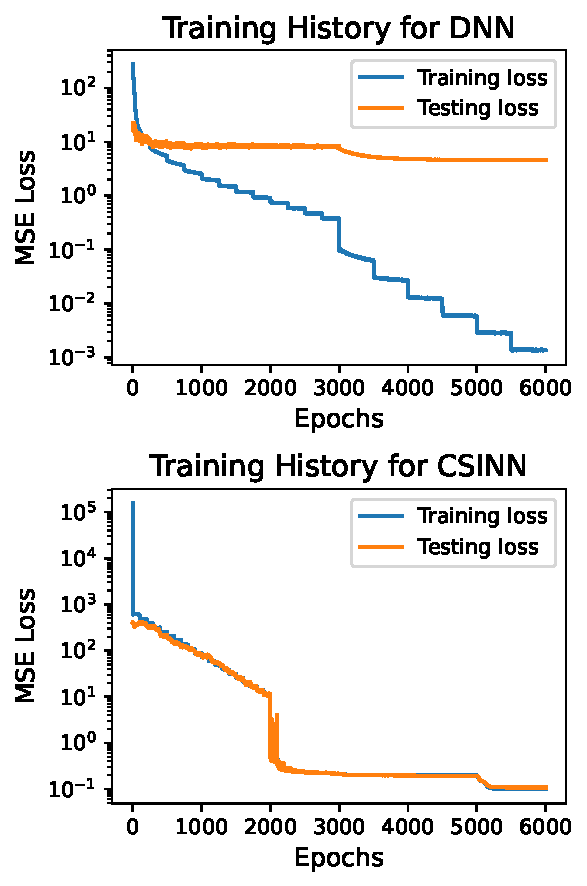
\includegraphics[width=0.85\linewidth]{figures/diagram-figure.pdf}
    \vspace{.05in}
    \caption{Our proposed approach for neural network-based optimality certification.}
    \label{fig:diagram}
\end{figure}
\section{Our Framework} \label{sec:approach}
{We propose this method as a certification meta-framework. It is distinct from a standalone solver in that it is not tied to a single convexification technique. Any convexification trick, valid inequality, or instance-specific lower bound methodology from the optimization literature can be applied within our framework. The core novelty is the mechanism that allows us to take any computationally expensive convex relaxation—whether exact or approximate—and convert it into a millisecond-scale verified proxy. This bridges the gap between high-dimensional convex geometry and real-time control.}

Consider a parametric optimization problem:
\vspace{-0.75em}
\begin{equation}
\begin{aligned}
    v(p) := ~\min_{x \in \mathbb{R}^n}~~~&f(x;p)  \\
    \text{s.t.}~~~~& g(x; p) \leq 0
\end{aligned} \label{eq:parametric_opt}
\vspace{-0.75em}
\end{equation}
in which the parameter $p \in \Phi \subseteq \mathbb{R}^d$ (where $\Phi$ is an arbitrary parameter set).
We assume that \eqref{eq:parametric_opt} is feasible for all $p \in \Phi$. The value function $v: \mathbb{R}^d \to \mathbb{R}$ expresses the globally optimal objective value as a function of the parameter $p$. The objective function $f(x;p)$ and/or the constraints $g(x;p)$ may be non-convex, so \eqref{eq:parametric_opt} may be a non-convex problem.

The value function may be used to test optimality of arbitrary feasible solutions. Given $\hat{x} \in \mathbb{R}^n$ that is feasible for \eqref{eq:parametric_opt}, if the cost $f(\hat{x};p) = v(p)$ then $\hat{x}$ is optimal; otherwise, if $f(\hat{x};p) > v(p)$, it is not.

Furthermore, \textit{approximations} of the value function may be used to test \textit{near}-optimality of arbitrary feasible solutions. Let $\hat{v}(p)$ be a function that approximates $v(p)$ over $\Phi$. If one can bound the approximation error of $\hat{v}(p)$ over $\Phi$, then they may also bound the optimality gap $f(\hat{x};p) - v(p)$ by comparing $f(\hat{x};p)$ to $\hat{v}(p)$. 

These observations motivate our work in this paper: we propose a machine learning framework to approximate the value functions of non-convex optimization problems for the purpose of approximate optimality certification. This framework may be especially beneficial in online settings, where obtaining exact optimality certificates may be expensive or impractical.

In particular, we propose to train a neural network to approximate $v(p)$ over the parameter set $\Phi$. 
We solve many instances of \eqref{eq:parametric_opt} for different $p \in \Phi$ to get training samples $(p_i, v(p_i))$ with $i$ ranging from $1$ to $N$.
The neural network $\hat{v}_{\theta}(p)$ is trained to minimize the mean-squared error loss:
\vspace{-0.5em}
\setlength{\jot}{0pt}
\begin{align}
    \min_\theta~ \frac{1}{N} \sum_{i=1}^{N} (v(p_i) - \hat{v}_{\theta}(p_i))^2
    \label{eq:learning-problem}
\end{align}
where $\theta$ represents the network's weights and biases.
If the trained neural network $\hat{v}_\theta(p)$ achieves low approximation error over the full parameter set $\Phi$, we may use it to certify near-optimality of solutions obtained via local search methods or other solvers. (Hereafter, we drop the `$\theta$' subscript notation for $\hat{v}(p)$ when referring to trained neural networks.)

The central challenge of learning to approximate the value function is developing a rich training data set. This is because evaluating $v(p)$ many times may be expensive, as it involves repeatedly solving a non-convex optimization problem.
This challenge may not always be easily overcome. However, for a large class of non-convex problems, convexification techniques allow us to find globally optimal solutions relatively efficiently. Therefore, the use of convexification techniques is a key element of our framework.

We now describe the role of convexification techniques within our framework. Consider a convex relaxation of problem \eqref{eq:parametric_opt}:
\begin{equation}
\begin{aligned}
    \tilde{v}(p) := ~\min_{x \in \mathbb{R}^n,~ u \in \mathbb{R}^k}~&\tilde{f}(x, u;p)  \\
    \text{s.t.}~~~~~& \tilde{g}(x, u; p) \leq 0
\end{aligned} \label{eq:convex_parametric_opt}
\end{equation}
where $\tilde{f}(x,u;p)$ and $\tilde{g}(x, u; p)$ are convex outer-approximations of $f(x;p)$ and $g(x; p)$, respectively, and $u \in \mathbb{R}^k$ are (optional) additional variables introduced to lift or convexify the problem.
Hereafter, we use $\tilde{v}(p)$ to denote the value function of any convex relaxation. Since \eqref{eq:convex_parametric_opt} is a convex relaxation of \eqref{eq:parametric_opt}, we have that $\tilde{v}(p) \leq v(p)$ for all $p \in \Phi$. Therefore, solving \eqref{eq:convex_parametric_opt} always yields a global lower bound on $v(p)$. When $\tilde{v}(p) = v(p)$, we say the relaxation is ``exact."

One may evaluate $v(p)$ in polynomial time by solving an \textit{exact} convex relaxation of \eqref{eq:parametric_opt}. This key insight enables our framework to be applied to any non-convex problem for which an exact or tight convex relaxation exists. By finding an exact convex relaxation of \eqref{eq:parametric_opt} for (almost) any $p \in \Phi$, one may solve problem instances of \eqref{eq:parametric_opt} relatively efficiently to develop a training data set for the learning problem \eqref{eq:learning-problem}.

%The tightest possible convex relaxation of \eqref{eq:epigraph_reformulation} is obtained by taking $\tilde{\mathcal{F}}(p) = \text{conv}(\mathcal{F}(p))$, i.e. the convex hull of $\mathcal{F}(p)$. However, this set is not easy to construct in general. Indeed, constructing the convex hull of $\mathcal{F}(p)$ may be just as hard as solving the original non-convex problem. 

As an important caveat, we note that convexification enables exact evaluation of $v(p)$ at the potential expense of slower computation due to the much larger size of the convexified problem.
This is precisely why we propose to use convexification techniques \textit{offline} to develop training data sets, and use neural networks \textit{online} to provide approximate optimality certificates.

\subsection{Convexification Techniques}

Convexification is a powerful approach for globally solving non-convex problems. The basic idea of convexification is to replace non-convex objectives or constraints with convex outer-approximations. The resulting convex problem is a relaxation of the original non-convex problem, and may be solved in polynomial time. The optimal value of the convex relaxation is a lower bound on the optimal value of the original problem. In some cases, an optimal solution of the original problem may be recovered from the convex relaxation, meaning the original problem may also be solved in polynomial time.

% Convexification has been used to tackle non-convex problems in a variety of domains. In combinatorial optimization, \citet{goemans1995improved} famously used semidefinite relaxation and randomization techniques to develop an approximate solution algorithm for the max-cut problem. \citet{sherali1990hierarchy} introduce a linear programming (LP) hierarchy to approximate the convex hull of 0-1 programming problems in higher dimensional spaces.
% \citet{bienstock2008approximate} constructs an approximate extended linear formulation of the 0-1 knapsack problem with a polynomial number of variables and constraints.
% The Lasserre hierarchy constructs a sequence of increasingly tight semidefinite relaxations of polynomial optimization problems \cite{lasserre2001global}. \citet{sojoudi2014exactness} provide sufficient conditions for the exactness of semidefinite and second-order cone relaxations of a large class of non-linear optimization problems. 
% In power systems, \cite{lavaei2012zero} propose a semidefinite relaxation of AC-OPF and provide sufficient conditions for exactness (see \citet{low2014convex} for a review of convex relaxations of AC-OPF). \citet{molzahn2016moment} study higher order semidefinite relaxations of AC-OPF, which are generally tighter but much larger and slower to solve. 

% Indeed, a common theme among convexification methods is that convexified problems may be orders of magnitude larger than the original non-convex problem, making these techniques cumbersome to use in online settings. 
% %For instance, to approximate the 0-1 knapsack polytope with $n$ items to within a factor of $\epsilon$, Bienstock (2004)'s extended linear formulation would require $\mathcal{O}(\epsilon^{-1}n^{1+\lceil 1/\epsilon \rceil})$ variables and $\mathcal{O}(\epsilon^{-1}n^{2+\lceil 1/\epsilon \rceil})$ constraints.
% For instance, for 0-1 programming problems in $\mathbb{R}^n$, the order-$d$ Sherali-Adams hierarchy LP has $\sum_{i=1}^{d}\binom{n}{i}$ variables.
% The SDP relaxation of a QCQP has $n(n+1)/2$ variables compared to $n$ variables in the original problem.
% For an arbitrary polynomial optimization problem in $\mathbb{R}^n$, the decision variable of the order-$d$ Lasserre hierarchy SDP is a $\binom{n+d}{d} \times \binom{n+d}{d}$ symmetric positive semidefinite matrix. High-order SDPs of the Lasserre hierarchy quickly become impractical to solve in real-time for even moderate-sized polynomial optimization problems. However, we claim that the power of convexification may be harnessed to \textit{learn} the value function of a non-convex problem \textit{offline} and thus provide optimality certificates.


\subsubsection{Structured QCQP} \label{sec:structured-QCQP}

Our method is highly compatible with structured QCQP, which is a class of QCQPs that exhibit specific structure -- either in the objective, the constraints, or both -- that can be exploited to make the problem easier to solve or analyze.

Many non-convex problems, including integer programming problems, may be exactly or approximately represented as polynomial optimization problems (POPs). A generic POP can be written as
\begin{equation}
\begin{aligned}
\min_{x \in \mathbb{R}^n}~& f(x) = \sum_\alpha f_\alpha x^\alpha \\
\text{s.t.}~~& g_i(x) =\sum_\alpha g_{i, \alpha} x^\alpha \geq 0, \quad i=1, \ldots, m
\end{aligned}
\label{eq:POP}
\end{equation}
where both the objective \( f(x) \) and constraints \( g_i(x) \) are polynomials in \( x \in \mathbb{R}^n \). We use the multi-index notation $x^\alpha:=x_1^{\alpha_1} \cdots x_n^{\alpha_n}$ for $x \in \mathbb{R}^n$ and $\alpha \in \mathbb{N}^n$.

Furthermore, a generic POP may be re-formulated via quadrification \citep{sherali2013reformulation, dalkiran2018linear} as a QCQP of the form
\begin{equation}
\begin{aligned}
    \min_{y \in \mathbb{R}^k}~& y^T M_0 y \\
    \text{s.t.}~& y^T M_i y \geq 0, \quad i = 1, 2, ..., l.
\end{aligned}
\label{eq:QCQP}
\end{equation}
Generally, this requires introducing new variables and constraints to re-write higher degree ($> 2$) monomials as quadratic terms. For example, the constraint `$3x^6 - 2x^2 \geq 0$' may be equivalently represented by the constraints `$y = x^2$, $~z = y^2$, and $3yz - 2y \geq 0$.'
As a result, the equivalent QCQP may be much larger than the original POP in terms of the number of variables ($k \gg n$) and constraints ($l \gg m$). 

Non-convex QCQPs are therefore a very broad class of optimization problem. Importantly, their simple structure has allowed for detailed study of QCQP convexification. In particular, a number of structural characterizations have been developed which are sufficient for exactness of the SDP relaxation of a QCQP:
\begin{equation}
\begin{aligned}
    \min_{Y \in \mathbb{R}^{n \times n}}~& \langle M_0, Y \rangle \\
    \text{s.t.}~~~& \langle M_i, Y\rangle \geq 0, \quad i = 1, 2, ..., l\\
    &~~ Y \succeq 0
\end{aligned}
\label{eq:SDP_relaxation}
\end{equation}
Examples of such structural characterizations include conditions on the number of constraints in \eqref{eq:QCQP}, such as the $S$-lemma \citep{boyd2004convex} and a number of more general results on low-rank SDP relaxations \citep{lemon2016low}. For example, the $S$-lemma proves the exactness of an SDP relaxation of a QCQP with a single quadratic constraint. Other examples include conditions on the underlying graph structure of the QCQP, as in \citet{sojoudi2014exactness} and \citet{bose2015quadratically}. For instance, if the underlying graph of a QCQP is acyclic, then its SDP relaxation must be exact. QCQPs with exact SDP relaxations may be solved efficiently, even if they have disconnected feasible regions or multiple local minima.

Additionally, exactness of the SDP relaxation of a QCQP may be ascertained not only \textit{a priori} via structural characterizations but also \textit{a posteriori} by proving feasibility of the optimal solution in the original problem. 
For example, exactness may ascertained from the rank of an optimal solution \citep{lemon2016low}. If $Y^*$ is optimal for the SDP relaxation \eqref{eq:SDP_relaxation} and $\text{rank}(Y^*) = 1$, then there exists a vector $x^* \in \mathbb{R}^n$ such that $Y^* = y^* y^{*T}$ and that is feasible (and thus optimal) for \eqref{eq:QCQP}. Therefore, whenever \eqref{eq:SDP_relaxation} is an exact relaxation of \eqref{eq:QCQP}, the minimum values of the two problems coincide and a globally optimal solution of \eqref{eq:QCQP} may be recovered from a solution of \eqref{eq:SDP_relaxation}. If there are multiple optimal solutions to \eqref{eq:SDP_relaxation}, it is possible that an optimal solution $Y^*$ obtained from an SDP solver is not rank-1 even though a rank-1 solution exists, in which case the optimal values agree anyways.

\subsubsection{QCQPs with Convex Value Functions}

Consider a QCQP parameterized by right-hand side uncertainty:
\begin{align}
    v(b) := \min_{y \in \mathbb{R}^k}~& y^T M_0 y \label{eq:QCQP_parametric} \\
    \text{s.t.}~& y^T M_i y \geq b_i, \quad i = 1, 2, ..., l \nonumber
\end{align}
As a minor point, we observe that if the parametric QCQP \eqref{eq:QCQP_parametric} admits an exact convex relaxation for all parameters $b \in \Phi$ where $\Phi \subseteq \mathbb{R}^m$ is some convex parameter set, then the value function $v(b)$ is convex over $\Phi$. The proof of this statement is trivial and follows the well-known argument for convexity of the value function of convex problems parameterized by right-hand side uncertainty.  However, the result is useful in practice. For instance, load-parameterized AC-OPF falls into this category of parametric QCQPs. The result also has implications for the \textit{types} of neural networks that can approximate the value functions of QCQPs.
\subsubsection{Sum-of-Squares and Lasserre Hierarchy}
Testing whether a polynomial \( f(x) \) is globally non-negative (\( f(x) \geq 0, \forall x \)) is NP-hard~\citep{murty1985some}. However, the sum of squares (SOS) decomposition provides a sufficient condition for non-negativity~\citep{parrilo2003semidefinite}. A polynomial \( p(x) \) is an SOS if there exist polynomials \( q_i(x) \) such that $p(x) = \sum_{i=1}^m q_i^2(x)$. 

Let $\Sigma[x]$ be the set of SOS polynomials, which forms a convex cone, and $\Sigma[x]_d$ be the set of SOS polynomials of degree at most $2 d$. A polynomial $\sigma(x) \in \Sigma_d[x]$ if it is of the form
\vspace{-1em}
\begin{equation}
\label{eq:SOS-d-def}
\sigma(x)=\sum_k\left(\sum_{|\alpha| \leqslant d} p_{k, \alpha} x^\alpha\right)^2 \text { where } p_{k, \alpha} \in \mathbb{R}.
\end{equation}
This is equivalent to the existence of $\left(\varphi_{\alpha, \beta}\right)_{|\alpha|,|\beta| \leqslant d} \succcurlyeq 0$ such that $\sum_{|\alpha| \leqslant 2 d} \sigma_\alpha x^\alpha=\sum_{|\alpha|,|\beta| \leqslant d} \varphi_{\alpha, \beta} x^{\alpha+\beta}$.
%(note that $\succcurlyeq$ is the positive semidefinite sign). 

Let $\mathbf{S}:=\left\{x \in \mathbb{R}^n \mid g_1(x) \geq 0, \ldots, g_m(x) \geq 0\right\}$, $\mathscr{M}(\mathbf{S})$ be the vector space of finite signed Borel measures supported on $\mathbf{S}$, and $\mathscr{M}_{+}(\mathbf{S})$ denote the cone of nonnegative elements of $\mathscr{M}(\mathbf{S})$. Problem~\eqref{eq:POP} can be reformulated as a linear program over probability measures~\citep{lasserre2015introduction}:

\begin{equation}
\min _{\mu \in \mathscr{M}_{+}(\mathbf{S})}\left\{\int_{\mathbf{S}} f \mathrm{~d} \mu: \int_S \mathrm{~d} \mu=1\right\}.
\label{eq:pop-measure}
\end{equation}

To make this reformulation tractable, we introduce the $r$-th order moment matrix $\mathbf{M}_r(y)$ associated with a sequence $y$, and the $r$-th order localizing matrix $\mathbf{M}_{r}\left(g_j y\right)$ associated with $y$ and constraint $g_j$:
\vspace{-0.5em}
\begin{equation}
\begin{aligned}
\mathbf{M}_r(y)&\coloneq\left(y_{\alpha+\beta}\right)_{|\alpha|,|\beta| \leqslant r}\\
\mathbf{M}_{r}\left(g_j y\right)&\coloneq(\sum_\gamma g_{i, \gamma} y_{\alpha+\beta+\gamma})_{|\alpha|,|\beta| \leqslant r}
\end{aligned}
\label{eq:Mr-def}
\vspace{-0.5em}
\end{equation}
We construct a hierarchy of moment relaxations for problem~\eqref{eq:pop-measure}, as $\mu \in \mathscr{M}_{+}(\mathbf{S})$ can be relaxed to $\mathbf{M}_{r-d_j}\left(g_j y\right) \succeq 0$, for all $j=0, \ldots, m$, and all $r \geq d_j=\left\lceil\operatorname{deg}\left(g_j\right) / 2\right\rceil$. Here, $\lceil\cdot\rceil$ denotes the ceiling function, and $\operatorname{deg}(\cdot)$ denotes the degree of a polynomial function.

Letting $r_{\min }\coloneq\max \left\{\lceil\operatorname{deg}(f) / 2\rceil, d_1, \ldots, d_m\right\}$, for $r \geq r_{\text {min }}$ of the hierarchy, we construct the order-$r$ moment SDP:
\begin{equation}
\begin{aligned}
\min _{y}\quad & L_{y}(f)  \\
\text { s.t. }\ \ \ &
\mathbf{M}_r(y) \succeq 0 \\
&  \mathbf{M}_{r-d_j}\left(g_j y\right) \succeq 0, \quad j =1,\dots,m \\
& y_0=1
\end{aligned}
\label{eq:pop-relax}
\end{equation}

\vspace{-1em}
where $L_{y}(f)\coloneq \sum_\alpha f_\alpha y^\alpha$, and $y \in \mathbb{R}^{\frac{(n+2r)\dots (n+1)}{(2r)!}}$. The dual of problem~\eqref{eq:pop-relax} is thus the following optimization problem over SOS polynomials of order $r$:
\vspace{-0.5em}
\begin{equation}
\label{eq:Lasserre-sos}
\begin{array}{cc}
\underset{\lambda, \sigma}\max & \lambda \\
\text { s.t. } & f-\lambda=\sigma_0+\sum_{k=1}^m \sigma_k g_k \\
& \lambda \in \mathbb{R}, \sigma_0 \in \Sigma_r[x], \\
& \sigma_i \in \Sigma_{r-d_j}[x], \quad j=1, \ldots, m .
\end{array}
\end{equation}
The Lasserre hierarchy, presented here, thus provides a sequence of SDP relaxations for solving the POP \eqref{eq:POP}. By defining $\mathcal{M}(\mathfrak{g})$ to be the quadratic module generated by $\mathfrak{g}$,  the following theorem provides a powerful condition for $\lambda$ to be a  lower bound on $f$.

\begin{theorem}[Putinar's Positivstellensatz~\citep{putinar1993positive}]
Assume that there exists $N>0$ such that $N-\|x\|_2^2 \in \mathcal{M}(\mathfrak{g})$ (Archimedean's condition). If $f$ is positive on $\mathbf{S}$, then
\vspace{-0.5em}
\begin{equation}
\label{eq:thm-sos}
f=\sigma_0+\sigma_1 g_1+\cdots+\sigma_m g_m,
\end{equation}
where $\sigma_0, \ldots, \sigma_m$ are SOS.
\vspace{-0.5em}
\end{theorem} 
Under the Archimedean condition, the hierarchy converges to the global optimum of the original problem as $r \to \infty$~\citep{lasserre2001global}. Importantly, the relaxation error is asymptotically bounded by $\mathcal{O}(1/r)$. For specific problem classes, such as those with a ball constraint, there is often no duality gap even at lower relaxation levels~\citep{josz2016strong}. In cases where basic relaxations ($r=1$) are insufficient or inexact, our framework naturally incorporates higher levels of the Lasserre hierarchy to tighten the bounds.

This flexibility allows for a strategic trade-off: one may choose a higher-order relaxation ($r \ge 2$) to reduce the relaxation gap $v(p) - \tilde{v}(p)$ and improve certificate quality, at the expense of increased offline computational cost for data generation. For instance, \citet{molzahn2016moment} demonstrate that while second-order relaxations for AC-OPF are tighter than first-order ones, they are significantly more expensive to solve. Our framework is agnostic to the chosen hierarchy level: it simply learns the value function $\tilde{v}(p)$ of a particular relaxation, which still provides a lower bound on $v(p)$ even when the relaxation is not exact.
\subsection{Illustrative Example} \label{subsec:illustrative_example}

\begin{figure}[ht!]
    \centering
    \begin{minipage}[t]{0.49\textwidth}
        \centering
        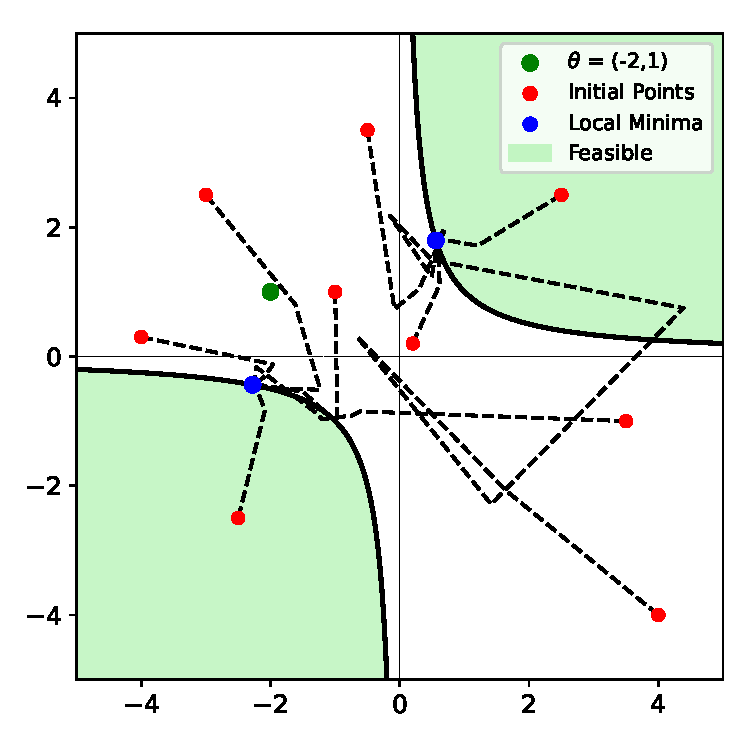
\includegraphics[width=\linewidth]{figures/QCQP_example_convergence.pdf}
        \caption{IPM convergence behavior for problem \eqref{eq:QCQP_example_prob} for $p = (-2,1)$. The global minimum is near $(-2.3, -0.5)$, while a spurious local minimum is near $(0.6, 1.8)$.}
        \label{fig:QCQP_example_fig}
    \end{minipage}
    \vspace{-0.5em}
    \hfill
    \begin{minipage}[t]{0.49\textwidth}
        \centering
        \includegraphics[width=\linewidth, trim=0 0 40 0]{figures/3d_value_function_plot_cropped.pdf}
        \caption{Neural network-based value function predictions over target parameter subspace $\Phi = [-5, 5] \times [-5, 5]$ for problem \eqref{eq:QCQP_example_prob}.}
        \label{fig:QCQP_vhat_fig}
    \end{minipage}
    \vspace{-0.5em}
\end{figure}

Let us illustrate our framework in a simple problem setting.
Consider the parametric QCQP over $x \in \mathbb{R}^2$:
\setlength{\jot}{2pt}
\begin{equation}
\begin{aligned}
    v(p) =~ \min_{x \in \mathbb{R}^2}~&(x_1 - p_1)^2 + (x_2 - p_2)^2 \\
    \text{s.t.}~& x_1 x_2 \geq 1
\end{aligned}
\label{eq:QCQP_example_prob}
\end{equation}

In words, the problem is to find a point of minimum squared distance to $p \in \mathbb{R}^2$ satisfying $x_1 x_2 \geq 1$. The quadratic constraint yields a non-convex feasible set with two disconnected regions. Therefore, any instance of this problem has two local minima.

As illustrated in Figure \ref{fig:QCQP_example_fig}, the convergence behavior of local search methods depends strongly on the initial point used in the search. Some initial points converge to the global minimum while others converge to the spurious local minimum. A naive strategy would be to try multiple initial points and keep the best solution found. However, without a principled strategy for selecting initial points, it is not clear whether this procedure will find the global minimum.

Consider solving the SDP relaxaton of problem \eqref{eq:QCQP_example_prob}. First, we re-write \eqref{eq:QCQP_example_prob} in compact matrix notation:
\setlength{\jot}{1pt}
\begin{equation}
\begin{aligned}
    v(p) = ~ \min_{y \in \mathbb{R}^3}~& y^T M_0 y \\
    \text{s.t.}~& y^T M_1 y \geq 1 \\
    &~y_1 = 1
\end{aligned}
\label{eq:QCQP_example_matrix}
\end{equation}
with $y := [1 ~~x^T]^T$ and
% \setlength{\abovedisplayskip}{6pt}
% \setlength{\belowdisplayskip}{7pt}
\begin{align*}
    \setlength{\arraycolsep}{1pt}
    M_0 = \begin{bmatrix}
        \|p\|_2^2 & -p_1 & -p_2 \\
        -p_1 & 1 & 0 \\
        -p_2 & 0 & 1
    \end{bmatrix}, \quad 
    \setlength{\arraycolsep}{8pt}
    M_1 = \begin{bmatrix}
        0 & 0 & 0 \\
        0 & 0 & \frac{1}{2} \\
        0 & \frac{1}{2} & 0
    \end{bmatrix}.
\end{align*}
The SDP relaxation of \eqref{eq:QCQP_example_prob} is:
%\setlength{\jot}{1pt}
\begin{equation}
\begin{aligned}
    \tilde{v}(p) = ~\min~&\langle M_0, Y \rangle \\
    \text{s.t.}~& \langle M_1, Y \rangle \geq 1 \nonumber \\
    & ~Y_{11} = 1 \\
    & ~Y \succeq 0
\end{aligned}
\label{eq:QCQP_example_SDP}
\end{equation}
The SDP relaxation is exact for all $p \in \mathbb{R}^2$ because \eqref{eq:QCQP_example_prob} has only one quadratic inequality constraint (see $S$-lemma; \citet{boyd2004convex}). 

Finally, we demonstrate the central proposition of this work: to train a neural network to approximate the value function of a non-convex optimization problem. We solved the SDP relaxation \eqref{eq:QCQP_example_SDP} for $5000$ instances of $p$ selected uniformly at random over $\Phi = [-5, 5] \times[-5,5]$ to obtain a data set of $(p, v(p))$ pairs.
%The exactness of the SDP relaxation for each instance of the parameter $p$ in the training data set was certified from the rank of the obtained optimal solution. Only a handful ($< 10$) of points in the training data failed this test. Interestingly, because the exactness of the SDP relaxation is known \textit{a priori}, every problem instance of \eqref{eq:QCQP_example_SDP} must have the same optimal objective function value as \eqref{eq:QCQP_example_prob} anyways ($\tilde{v}(p) = v(p)$). 
The trained neural network predictions are shown in Figure \ref{fig:QCQP_vhat_fig}. The neural network achieved $\mathbf{0.01\%}$ \textbf{average} / $\mathbf{0.78\%}$ \textbf{maximum} prediction error over the test data set of 1500 points. The trained neural network can thus reliably certify near-optimality of solutions of \eqref{eq:QCQP_example_prob}.

\section{Experiments} \label{sec:experiments}

We now present results from several experiments in which we applied our approach to non-convex optimization problems from power systems, digital communications, and integer programming.
The purpose of these experiments is to demonstrate the viability of our framework in diverse problem settings.
Additional information and details may be found in Appendix \ref{sec:experiments-details}.

\subsection{Input-Convex and Scale-Invariant Neural Networks}

In each experiment, we trained neural networks to approximate the value functions of parametric optimization problems. In some cases, the value functions possess geometric properties like convexity and scale invariance (positive homogeneity) that may also be enforced in the neural networks, for example, by constraining the weights and biases of the network to take certain values (see Appendix \ref{app:nn-architecture}). 

While our framework does not require convex or scale invariant value functions, these properties may be exploited to provide better performance guarantees. In particular, input-convex neural networks (ICNNs) \citep{pmlr-v70-amos17b} have relatively strong performance guarantees compared to generic deep neural networks (DNNs) for approximating convex functions \cite{rosemberg2024learning}. Throughout our experiments, we explored ICNNs' ability to approximate convex value functions. We also prove novel error bounds and performance guarantees for ICNNs in Appendix \ref{app:icnn-guarantees}.

\subsection{Power Systems Optimization}

The alternating current optimal power flow (AC-OPF) problem is solved by power system operators approximately every 5 minutes to minimize cost while balancing demand and generation. It is one of the most fundamental optimization problems in power systems. AC-OPF explicitly represents the steady-state physics of AC electricity networks, which are expressed as nonlinear equations relating nodal voltages and power injections (see formulation in Appendix \ref{sec:experiments-details}). These yield quadratic equality constraints in the formulation, which makes AC-OPF a special case of non-convex QCQP.

\citet{lavaei2012zero} derive a sufficient condition for exactness of the SDP relaxation of AC-OPF, which holds for many real-world power systems. However, solving the SDP relaxation of AC-OPF is often much slower than using machine learning-based solvers or local search methods, especially in large power systems. SDP relaxation is thus seldom used in real-time power system operations. However, by learning to approximate the value function of the SDP relaxation of AC-OPF, one may obtain optimality certificates for faster solvers which lack optimality guarantees on their own. This is the motivation for our experiment.

\begin{table*}[t]
\centering
\caption{Results of AC-OPF experiments. Value function approximation error for DNNs and ICNNs for different IEEE cases and experiment configurations. Results with $<0.01\%$ error are marked with a long dash ``---."}
%\begin{adjustbox}{width=\textwidth}
\begin{tabular}{*{3}{c} *{6}{c}}
\toprule
\textbf{IEEE Case} & \textbf{Data Dim.} & \textbf{\# Samples} &
\multicolumn{2}{c}{\textbf{Avg. Pct. Error}} &
\multicolumn{2}{c}{\textbf{Max. Pct. Error}} \\
\cmidrule(lr){4-5} \cmidrule(lr){6-7}
& & & \textbf{DNN} & \textbf{ICNN} & \textbf{DNN} & \textbf{ICNN} \\
\midrule
\texttt{ieee9}   & 1  & 5000  & ---      & ---            & $0.02\%$ & $0.01\%$       \\
         & 3  & 5000  & ---      & ---            & $0.55\%$ & $1.25\%$       \\
         & 6  & 10000 & $0.04\%$ & ---            & $2.22\%$ & $4.19\%$       \\
\addlinespace \hline \addlinespace
\texttt{ieee14} & 3  & 5000  & ---      & ---            & $0.54\%$ & $1.62\%$       \\
         & 6  & 10000 & ---      & ---            & $0.53\%$ & $2.43\%$       \\
         & 10 & 20000 & ---      & ---            & $0.21\%$ & $0.41\%$       \\
\addlinespace \hline \addlinespace
\texttt{ieee30}  & 6  & 10000 & ---      & ---            & $0.39\%$ & $1.04\%$       \\
         & 10 & 20000 & ---      & ---            & $0.26\%$ & $0.90\%$       \\
         & 25 & 50000 & ---      & ---            & $0.13\%$ & $0.58\%$       \\
\addlinespace \hline \addlinespace
\texttt{ieee118} & 10 & 20000 & $0.03\%$ & ---            & $0.96\%$ & $0.29\%$       \\
         & 25 & 50000 & ---      & ---            & $0.13\%$ & $0.53\%$       \\
\addlinespace \hline \addlinespace
\texttt{ieee300} & 60 & 30000 & ---      & ---            & $0.55\%$ & $0.53\%$    \\
\bottomrule
\end{tabular}
%\end{adjustbox}
\label{tab:ACOPF-results}

\end{table*}

For several IEEE test power systems, we trained DNNs and ICNNs to approximate the value function of AC-OPF parameterized by real and reactive load at each bus. We obtained training and testing data by solving exact SDP relaxations of AC-OPF. The DNN and ICNN models achieved very low approximation error in our experiments. Maximum error was less than 2-3\% in most experiments, and average error was near-zero. 
%For reference, the prediction targets (optimal objective function values) in our test data sets had coefficients of variation between 8\% and 45\%, meaning the neural networks achieved good performance relative to the size of the variance of the data. 
Furthermore, the approximation error was relatively consistent across test cases of widely varying size and data dimension, which indicates that our approach can scale well to larger power systems.
%In our experiments, IPOPT never converged to a spurious local minimum, though in many instances (30\%) of the \texttt{ieee300} case it outright failed to converge to a feasible solution.
%This highlights the sensitivity of local search methods to the choice of initial point in non-convex problems.
Furthermore, our timing comparison results (Table \ref{tab:method-time}) show unsurprisingly that neural network inference is orders of magnitude faster than solving AC-OPF via convexification or local search. Overall, the results suggest that neural networks can quickly and reliably certify optimality of AC-OPF solutions.

\subsection{Digital Communications}

The MIMO detection problem, which is an instance of QCQP with complex variables, arises in many signal processing applications. Typically, MIMO detection must be solved for rapidly time-varying signal and channel parameters. Although convexification methods like SDP relaxation have been used to solve MIMO detection, they are typically too slow to be used in practice. Several heuristics have been developed to approximately (sub-optimally) solve MIMO detection in realistic online settings. In \citet{samuel2017deep}, the authors developed a machine learning-based solver for the MIMO detection problem, which achieved good performance. However, heuristic and machine learning-based approaches lack optimality guarantees and may benefit from neural network optimality certificates.

%The value function $\tilde{v}(y)$ is neither convex nor scale invariant, and therefore we did not attempt to train an ICNN or SINN to learn the value function in our experiments. 
We solved 5000 instances of the SDP relaxation of MIMO detection with randomly generated noisy signals $\bar{y}$. We certified the exactness of each SDP instance by testing whether a rank-1 solution was obtained. 
%None of the problem instances failed this test. 
We trained a DNN to approximate the value function using the Adam optimizer with a learning rate of 0.01 over 3000 epochs. The trained DNN achieved near-zero training loss, and $\mathbf{0.3\%}$ \textbf{average / }$\mathbf{2.5\%}$ \textbf{maximum} error over the test data set of $1500$ points. The trained DNN can therefore reliably certify optimality of detected digital signals.

\subsection{Integer Programming}


{
\setlength{\tabcolsep}{10pt}
\begin{table}[t]
\centering
\caption{Time to solve or predict the optimal cost of 100 AC-OPF instances of \texttt{ieee300}. Experiments were conducted on a 2024 MacBook Air equipped with an 8-core Apple M3 chip and 8 GB of unified memory.}
\begin{tabular}{lcc}
\hline
\textbf{Problem} & \textbf{Software} & \textbf{ Time} \\
\hline
AC-OPF SDP & CVXOPT & 30m 55s \\
AC-OPF & IPOPT &9m 3s  \\
DNN Inference & PyTorch & 0.1s \\
\hline
\end{tabular}
\label{tab:method-time}

\end{table}
}
\setlength{\tabcolsep}{3pt} 
\begin{table}[t]
\centering
\caption{Results of 0-1 knapsack experiments. Each block shows the results of a different set of experiments.}
\begin{tabular}{lcc}
\multicolumn{3}{c}{\textbf{10 Item Knapsack}:  data dim. = 5,~ \# samples = 50000}\\
\midrule
\textbf{Network~~} & \textbf{Avg. Pct. Error} & \textbf{Max. Pct. Error} \\
\midrule
DNN   & 0.27\% & 2.29\% \\
ICNN  & 0.02\% & 2.12\% \\
SINN  & 0.30\% & 3.87\% \\
CSINN & \textbf{0.01\%} & \textbf{0.56\%} \\
\addlinespace
\addlinespace
\multicolumn{3}{c}{\textbf{30 Item Knapsack}: data dim. = 8,~ \# samples = 80000} \\
\midrule
\textbf{Network~~} & \textbf{Avg. Pct. Error} & \textbf{Max. Pct. Error} \\
\midrule
DNN   & 1.32\% & 8.88\% \\
ICNN  & \textbf{0.10\%} & \textbf{0.92\%} \\
SINN  & 1.20\% & 15.67\% \\
CSINN & 0.50\% & 5.02\% \\
\bottomrule
\end{tabular}
\vspace{-1em}
\label{tab:knapsack-results}

\end{table}

In this experiment, we trained neural networks to certify optimality of the 0-1 knapsack problem parameterized by the cost vector $c \in \mathbb{R}^n_+$. We solved thousands of problem instances using Gurobi's mixed-integer linear program solver \citep{gurobi} to obtain data sets for our experiments. We trained a variety of neural network architectures, including DNNs, ICNNs, and scale-invariant and convex scale-invariant networks (SINNs and CSINNs) to approximate the value function. We measured the average and maximum approximation error of each network in each experiment.
The results are summarized in Table \ref{tab:knapsack-results}.

The average performance of ICNNs and CSINNs was substantially better than DNNs and SINNs, indicating that special neural network architectures can reduce overfitting and improve performance.
The good performance of ICNNs and CSINNs in our experiments highlights the potential to integrate neural networks into other solvers. For example, neural networks may be used to certify optimality of linear relaxations of integer programs, or speed branch-and-bound by pruning branches whose objective function value exceeds the network's prediction by a pre-determined threshold.

% Since $v(c)$ is scale invariant (i.e. positively homogeneous), by Euler's theorem it also satisfies
% {
% \setlength{\abovedisplayskip}{6pt}
% \setlength{\belowdisplayskip}{6pt}
% \setlength{\jot}{0pt}
% \setlength{\arraycolsep}{3pt}
% \begin{align*}
%     v(c) = \nabla v(c)^Tc
% \end{align*}
% }
% Let $x^*(c)$ denote an optimal solution of \eqref{eq:knapsack}, which we assume to be unique. Note that for a particular $i \in \{1, ..., n\}$, we have
% {
% \setlength{\abovedisplayskip}{5pt}
% \setlength{\belowdisplayskip}{8pt}
% \setlength{\jot}{0pt}
% \setlength{\arraycolsep}{3pt}
% \begin{align*}
% \nabla v(c)_i =
% \begin{cases}
% 1 & \text{if } x^*(c)_i = 1, \\
% 0 & \text{if } x^*(c)_i = 0.
% \end{cases}
% \end{align*}
% }
% Therefore, $\nabla v(c) = x^*(c)$ for all $c \in \mathbb{R}^n_+$ such that the corresponding instance of \eqref{eq:knapsack} has a unique solution. Furthermore, if a SINN $\hat{v}(c)$ can approximate the value function to within $\epsilon$ error for all $c \in \Phi \subset \mathbb{R}^n_+$, then
% \begin{align*}
%     |\hat{v}(c) - v(c)| &= \|\nabla \hat{v}(c)^Tc - \nabla v(c)^T c \| \\
%     &\leq \| \nabla \hat{v}(c) - \nabla v(c) \| \cdot \| c\| \leq \epsilon \\
%     \implies& \| \nabla \hat{v}(c) - x^*(c) \| \leq \frac{\epsilon}{\|c\|}
% \end{align*}
% for all $c \in \Phi$ such that $x^*(c)$ is a unique optimal solution of \eqref{eq:knapsack}.
% In other words, by learning to approximate the scale invariant value function of \eqref{eq:knapsack} with a SINN, the gradient of the value function (and therefore an approximate optimal solution mapping) may be indirectly learned as well. The error may also depend on the norm of the cost vector $c$, with larger values of $\|c\|$ generally being preferred. However, due to noise in the training process, the gradient estimator of the trained SINN $\nabla \hat{v}(c)$ is typically not in $\{0, 1\}^n$, and therefore may need to be rounded or projected to obtain feasible a solution to \eqref{eq:knapsack}. Therefore, we propose the following simple approach to compute approximate solutions of the parametric 0-1 knapsack problem using SINNs.
% \begin{algorithm}[H]
% \caption{Approximate 0-1 Knapsack via CSINN}
% \label{alg:approx-knapsack}
% % Unnumbered input/output
% \begin{algorithmic}[0]
% \STATE \textbf{Input:} CSINN $\hat{v}(c)$, cost vector $c \in \mathbb{R}^n$
% \STATE \textbf{Output:} Approximate solution $\hat{x} \in \{0,1\}^n$
% \end{algorithmic}
% % Numbered steps
% \begin{algorithmic}[1]
% \STATE Normalize cost vector: $\hat{c} \gets c / \|c\|$
% \STATE Compute CSINN gradient: $\hat{g} \gets \nabla \hat{v}(\hat{c})$
% \STATE Round to integer solution: $\hat{x} \gets \mathbf{1}(\hat{g} > 0.5)$
% \STATE Ensure feasible solution:
% \end{algorithmic}
% \begin{algorithmic}[0]
% \WHILE{$w^T \hat{x} > b$}
%     \STATE $k \gets \argmin_i \{ \frac{c_i}{w_i} : \hat{x}_i = 1 \} $ \\
%     \STATE $\hat{x}_k \gets 0$
% \ENDWHILE
% \end{algorithmic}
% \end{algorithm}
% This approach may be further improved by using techniques such as Sobolev training \cite{czarnecki2017sobolev}, in which neural networks are trained to approximate both a function's value and its derivatives. It is similar in spirit to the ICNN-based DC-OPF solver developed in \citet{zhang2021convex}, which uses first-order information about the value function to recover optimal solutions from the trained ICNN. However, our algorithm takes advantage of scale invariance of the neural network architecture and does not penalize the gradient error during training. 
% Remarkably, our approximate knapsack solver achieves good performance over the test data set despite never observing optimal knapsack solutions during training. The average (maximum) optimality gap of the CSINN-based solutions was $1.7\%$ ($51.4\%$). The solver returned the globally optimal solution in $78\%$ of test set problem instances.
% Overall, these experiments suggest an interesting new approach to learning optimal solution mappings for 0-1 knapsack and other MILPS.

\section{Conclusion} \label{sec:conclusion}
In this work, we proposed an innovative framework for real-time optimality certification in non-convex optimization tasks.
Our framework leverages convexification techniques and machine learning to learn the optimal value function of parametric optimization problems.
{By functioning as a meta-framework, our method is compatible with various convexification schemes, including the Lasserre hierarchy for general polynomial optimization, as well as various fast solvers.} By training neural networks to approximate the optimal value of a convex relaxation, we shift the computational burden from real-time optimization to offline training. Under suitable conditions, the convex relaxation provides a tight lower bound on the original non-convex problem, so candidate solutions that are sufficiently close to the predicted optimal value are assured to be near-globally optimal.
Our proposed framework not only expands the applicability of convexification methods to online optimization, but also offers a new conceptual approach to apply learning-based performance guarantees to fast heuristic solvers.
%This methodology not only improves computational efficiency but also offers a theoretical framework for achieving global optimality in previously intractable non-convex optimization tasks. 
Future work will focus on refining machine learning-based optimality certification and extending this approach to more diverse classes of non-convex problems.






\section{Preparing PostScript or PDF files}

Please prepare PostScript or PDF files with paper size ``US Letter'', and
not, for example, ``A4''. The -t
letter option on dvips will produce US Letter files.

Consider directly generating PDF files using \verb+pdflatex+
(especially if you are a MiKTeX user).
PDF figures must be substituted for EPS figures, however.

Otherwise, please generate your PostScript and PDF files with the following commands:
\begin{verbatim}
dvips mypaper.dvi -t letter -Ppdf -G0 -o mypaper.ps
ps2pdf mypaper.ps mypaper.pdf
\end{verbatim}

\subsection{Margins in LaTeX}

Most of the margin problems come from figures positioned by hand using
\verb+\special+ or other commands. We suggest using the command
\verb+\includegraphics+
from the graphicx package. Always specify the figure width as a multiple of
the line width as in the example below using .eps graphics
\begin{verbatim}
   \usepackage[dvips]{graphicx} ...
   \includegraphics[width=0.8\linewidth]{myfile.eps}
\end{verbatim}
or % Apr 2009 addition
\begin{verbatim}
   \usepackage[pdftex]{graphicx} ...
   \includegraphics[width=0.8\linewidth]{myfile.pdf}
\end{verbatim}
for .pdf graphics.
See section~4.4 in the graphics bundle documentation (\url{http://www.ctan.org/tex-archive/macros/latex/required/graphics/grfguide.ps})

A number of width problems arise when LaTeX cannot properly hyphenate a
line. Please give LaTeX hyphenation hints using the \verb+\-+ command.

\subsubsection*{Broader Impact Statement}
In this optional section, TMLR encourages authors to discuss possible repercussions of their work,
notably any potential negative impact that a user of this research should be aware of. 
Authors should consult the TMLR Ethics Guidelines available on the TMLR website
for guidance on how to approach this subject.

\subsubsection*{Author Contributions}
If you'd like to, you may include a section for author contributions as is done
in many journals. This is optional and at the discretion of the authors. Only add
this information once your submission is accepted and deanonymized. 

\subsubsection*{Acknowledgments}
Use unnumbered third level headings for the acknowledgments. All
acknowledgments, including those to funding agencies, go at the end of the paper.
Only add this information once your submission is accepted and deanonymized. 

\bibliography{main}
\bibliographystyle{tmlr}

\appendix

\section{Additional Background} \label{sec:additional_background}

\subsection{Machine Learning-Based AC-OPF Solvers}

Using machine learning to assist in optimization has garnered strong interest in power systems research. Notably, several works contribute machine learning-based AC-OPF solvers, motivated by the growing need to solve large-scale problem instances with time-varying load and renewables \citep{van2021machine, jiang2024advancements}. While practical experience and some theoretical work has shown that spurious local minima may be rare in AC-OPF, it remains an interesting and potentially important challenge to solve AC-OPF efficiently using machine learning tools \citep{zhou2021conditions}. There are also several well-known examples of AC-OPF problems with spurious local solutions \citep{bukhsh2013local}.

Many machine learning-based solvers, including those developed by \citet{pan2021deepopf} and \citet{singh2021learning}, directly map load and renewables to optimal AC-OPF solutions. \citet{zhang2022learning} use a Lagrangian duality-based approach to learn solution mappings in a more favorable optimization landscape. \citet{zhang2021convex} train input-convex neural networks (ICNNs) to learn the value function of parametric DC-OPF, and exploit linear programming duality to recover optimal solutions from the network predictions. \citet{deka2019learning} train neural networks to classify active constraint sets of DC-OPF problems, from which optimal solutions may be efficiently computed. \citet{baker2019learning} uses machine learning-predicted AC-OPF solutions as warm starts for local search solvers. \citet{rosemberg2024learning} train ICNNs to learn the value function of AC-OPF, though they did not use convexification techniques to certify the optimality of AC-OPF solutions.

%Machine learning-based solvers have also been developed for other canonical problems in power systems. \citet{chen2020input} use ICNNs to assist in voltage regulation in distribution networks, and \citet{christianson2024fast} use ICNNs to screen contingency scenarios in security-constrained DC-OPF. \citet{pineda2022learning} propose machine learning methods to solve unit commitment problems, and \citet{pineda2024learning} apply machine learning to optimal transmission switching.

Though many of these approaches achieve good performance, they still lack optimality guarantees (and even feasibility guarantees in some cases). Solutions obtained from machine learning-based solvers must often be projected into the feasible set in a final step. A key challenge is that solution mappings are high dimensional and discontinuous functions that are difficult to approximate \citep{pan2022deepopf}. Certifying optimality of solutions obtained from machine learning-based solvers therefore remains an important challenge.

\subsection{Special Neural Network Architectures} \label{app:nn-architecture}
For certain non-convex problems, the value function is convex and/or positive homogeneous. This is not always the case, even for non-convex problems which admit exact convex relaxations. However, when this is the case, it is conceivably desirable to enforce these properties in a neural network trained to approximate the value function. Therefore we turn our attention to input-convex and scale-invariant neural networks (ICNNs and SINNs), which are special neural network architectures that respectively enforce convexity and positive homogeneity in the network outputs \citep{pmlr-v70-amos17b, bamberger2025approximating}.
% An ICNN is a type of neural network designed to ensure that the output is a convex function of the input~\cite{pmlr-v70-amos17b}. This property is enforced directly in the neural network architecture by restricting certain neural activation functions to be convex and non-decreasing. 
\begin{figure}[H]
    \centering
    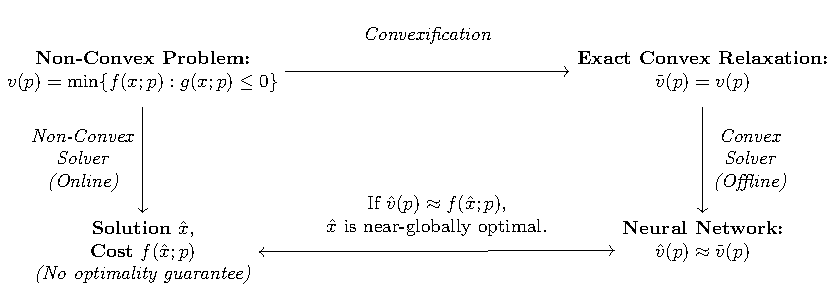
\includegraphics[width=0.7\linewidth]{figures/icnn-figure.pdf}
    \caption{Neural network with skip connections.}
    \label{fig:icnn}
\end{figure}
Consider a $k$-layer neural network with skip connections and input $y \in \mathbb{R}^d$. For $i=0,\ldots,k-1$ we have
\setlength{\abovedisplayskip}{7pt}
\setlength{\belowdisplayskip}{7pt}
\begin{equation*}
    z_{i+1} = \sigma_i\left(W^{(z)}_i z_i + W^{(y)}_i y + b_i \right ), \;\; h(y;\theta) = z_k
\end{equation*}
% \vspace{-0.5em}
% \begin{equation}
% \begin{split}
% \label{eq-ficnn}
% %z_1 & = g_0\left(W^{(xy)}_0 \xy + b_0 \right) \\
% z_{i+1} & = \sigma_i\left(W^{(z)}_i z_i + W^{(y)}_i y + b_i \right ), \;\; h
% (y;\theta) = z_k
% \end{split}
% \vspace{-0.5em}
% \end{equation}
where $z_i$ denotes the activation or output of layer $i$, $\theta = \{W^ {(y)}_{0:k-1}, W^{(z)}_{1:k-1}, b_{0:k-1}\}$ are the neural network weights and biases, and $\sigma_i$ are nonlinear activation functions (we define $z_0 = 0$ and $W^{(z)}_0 = 0$ in the input layer). Here, $W^{(z)}_i$ are feedforward connection weights while $W_i^{(y)}$ are skip connection weights and $b_i$ are layer biases. 

By imposing certain conditions on the activation functions and weights and biases, the function $h(y;\theta)$ can be made to be convex or scale invariant in $y$. In particular:
\begin{enumerate}
    \item \textbf{ICNN}: The function $h(y;\theta)$ is convex in $y$ if all feedforward connection weights $W_{1: k-1}^{(z)}$ are non-negative and all activation functions $\sigma_i$ are convex and non-decreasing \citep{pmlr-v70-amos17b}. That is, for all $y_1, y_2 \in \mathbb{R}^d$, $\lambda \in [0, 1]$, we have \[
    h(\lambda y_1 + (1 - \lambda) y_2; \theta) \leq \lambda h(y_1; \theta) + (1 - \lambda) h(y_2; \theta) \]
    \item \textbf{SINN}: The function $h(y;\theta)$ is scale invariant (positively homogeneous) if all biases $b_i$ are zero and all activation functions $\sigma_i$ are scale invariant \citep{bamberger2025approximating}. That is, for all $y \in \mathbb{R}^d$, $\lambda \geq 0$, we have \[h(\lambda y; \theta) = \lambda h(y; \theta)\]
\end{enumerate}

By enforcing these properties in the neural network architecture, ICNNs and SINNs provide strong inductive bias for learning to approximate convex or positive homogeneous functions. They may achieve lower generalization error and their outputs may be easier to interpret and integrate into optimization frameworks.

The ReLU activation function ($\text{ReLU}(x) = \max \{0, x\}$) is convex, non-decreasing, and scale invariant, and therefore can be used in both ICNNs and SINNs.

\section{Experiment Details} \label{sec:experiments-details}

\subsection{Training Neural Networks}

Throughout our experiments, we trained deep neural networks to approximate the value functions of non-convex problems. We used a 6-layer architecture whose input dimension $d$ varied by experiment. The five hidden layers had progressively fewer neurons: 512, 512, 256, 64, and 16 neurons. The output layer had a single neuron. For ICNN architectures, skip connections were included between the input layer and hidden layers, while DNNs and SINNs did not have skip connections. However, the number of layers and neurons in each network was the same regardless of architecture.

To train the neural networks we used a two-stage approach: first, we trained the DNN with stochastic gradient descent (SGD) for 1000-5000 epochs, followed by 1000-5000 epochs of training with Adam. We adopted this two-stage approach because it seemed to be more stable than using either SGD or Adam by itself. 
The batch size during training ranged from 30-200 samples, and the total size of the data varied between 5000 and 100000 samples in our experiments. 
In all experiments, the data were split into training (70\%) and test (30\%) data sets.
Our goal was to achieve zero training loss.

When training ICNNs and SINNs, the training process was modified. For SINNs, we clamped all biases $b_i$ to zero. For ICNNs, the feedforward connection weights $W^{(z)}_i$ were clipped to be nonnegative after every training iteration. Implementing the clipping step required careful tuning of learning rates to avoid slow convergence (generally, larger learning rates were used to train ICNNs).

\subsection{Power Systems Optimization}


We trained neural networks to approximate the value function of AC-OPF parameterized by real and reactive load for several IEEE test power systems (see Table \ref{tab:ieee-description}). Our experimental procedure, which we repeated for each test system, was as follows.

For a given IEEE test power system with $n$ buses, let $P^{MAX}_D, Q^{MAX}_D \in \mathbb{R}^n$ be vectors of the nominal real and reactive load at each bus. We randomly sampled real and reactive load vectors $P_D, Q_D$ from $\Phi \subseteq [0, P^{MAX}_D] \times [0, Q^{MAX}_D] \subset \mathbb{R}^{2n}$ and solved the corresponding SDP relaxation of AC-OPF for each instance to obtain the relaxed optimal cost $\tilde{v}(P_D, Q_D)$. In particular, we solved the SDP relaxation in \citet{lavaei2012zero} using the solver in \citet{madani2014sdp}. Exactness of each SDP relaxation was ascertained \textit{a posteriori} from the rank of the obtained optimal solution. Any problem instance for which a rank-1 solution was not obtained was discarded from the data set. (These instances made up fewer than $5\%$ of samples in all of our experiments.) The valid samples were split into training (70\%) and test (30\%) data sets. A deep neural network (DNN) and input-convex neural network (ICNN) were separately trained to approximate the value function $v(P_D, Q_D)$. We measured the average and maximum percentage error of the DNN and ICNN predictions over the test data set. 
%For comparison, we also solved each test data set problem instance with the interior point solver IPOPT \citep{wachter2006implementation}.
Experiment configurations and results are reported in Table \ref{tab:ACOPF-results}.

An important detail of our experiments is that real and reactive load were not sampled from the full-dimensional parameter space. In real power systems, electricity demand at different buses is correlated, and the load data may lie in or near a low-dimensional subspace of the ambient space. For instance, in a system with $n$ load buses, the ambient space has $2n$ dimensions, but the data may lie in an $m$-dimensional subspace of $\mathbb{R}^{2n}$ with $m \ll 2n$. We therefore chose to vary the intrinsic dimension of the load data in our experiments (the intrinsic data dimension in each experiment is given in the ``data dim." column in Table \ref{tab:ACOPF-results}). We hypothesized that neural networks would achieve better performance on data with lower intrinsic dimension . For each test system, we tested multiple configurations of the intrinsic data dimension and number of samples. In each experiment, real and reactive load data was uniformly sampled from a randomly chosen $m$-dimensional subspace $\Phi \subseteq [0, P^{MAX}_D] \times [0, Q^{MAX}_D] \subset \mathbb{R}^{2n}$.

Let us now write the AC-OPF formulation. Consider a power network with a set of buses $\mathcal{N} = \{1, 2, ..., n\}$, set of generator buses $\mathcal{G} \subseteq \mathcal{N}$, and set of lines $\mathcal{L} \subseteq \mathcal{N} \times \mathcal{N}$. We define the variables, parameters, and expressions associated with bus $k \in \mathcal{N}$ as follows:
\begin{itemize}[itemsep=2pt, topsep=0pt, parsep=0pt, partopsep=0pt]
    \item $V_k = V_{dk} +\mathbf{j} V_{qk}$: Apparent (real and reactive) voltage.
    \item $P_{Dk} + \mathbf{j} Q_{Dk}$: Real and reactive power demand or load.
    \item $P_{Gk} + \mathbf{j} Q_{Gk}$: Real and reactive power generation.
    \item $f_{Ck}(P_{Gk}) = c_{k2} P_{Gk}^2 + c_{k1} P_{Gk} + c_{k0}$: Convex quadratic cost function of real power generation.
    \item $f_{Vk}(V_d, V_q) = V_{dk}^2 + V_{qk}^2$: Squared voltage magnitude.
\end{itemize}

Let $\mathbf{Y} = \mathbf{G} + \mathbf{jB}$ be the bus admittance matrix of an equivalent $\Pi$ circuit model of the network.
The real and reactive power generation at each bus are related to the bus voltages through the power flow equations $P_{Gk} := f_{Pk}(V_d, V_q)$ and $Q_{Gk} := f_{Qk}(V_d, V_q)$, where
{
\setlength{\abovedisplayskip}{1pt}
\setlength{\belowdisplayskip}{3pt}
\setlength{\jot}{0pt}
\setlength{\arraycolsep}{3pt}
\begin{align}
    f_{Pk} :=  P_{Dk} + &V_{dk} \sum_{i=1}^{n}(\mathbf{G}_{ki} V_{di} - \mathbf{B}_{ki} V_{qi})
    + V_{qk} \sum_{i=1}^n (\mathbf{B}_{ki} V_{di} + \mathbf{G}_{ki} V_{qi}) \label{eq:active-power-flow}\\
    f_{Qk} := Q_{Dk} + &V_{dk}\sum_{i=1}^{n}(-\mathbf{B}_{ki} V_{di} - \mathbf{G}_{ki} V_{qi})
    + V_{qk} \sum_{i=1}^n (\mathbf{G}_{ki} V_{di} - \mathbf{B}_{ki} V_{qi}) \label{eq:reactive-power-flow}
\end{align}
}

We may write AC-OPF parameterized by real and reactive power demand $P_D$ and $Q_D$ as follows:
\begin{align}
    v(P_D, Q_D) := ~ \min~& \sum_{k \in \mathcal{G}} f_{Ck}(f_{Pk}(V_d, V_q))  \label{eq:AC-OPF} \\
    \text{s.t.}~& P_{Gk}^{min} \leq f_{Pk}(V_d, V_q) \leq P_{Gk}^{max} \label{constr:max-real-power} \\
    & Q_{Gk}^{min} \leq f_{Qk}(V_d, V_q) \leq Q_{Gk}^{max} \label{constr:max-reactive-power}\\
    & (V_{k}^{min})^2 \leq f_{Vk}(V_d, V_q) \leq (V_{k}^{max})^2 \label{constr:voltage-mag} \\
    & V_{q0} = 0 \label{constr:slack-bus}
\end{align}
where constraints are defined for all buses $k \in \mathcal{N}$. Constraints \eqref{constr:max-real-power} and \eqref{constr:max-reactive-power} bound the real and reactive power output at each bus; constraint \eqref{constr:voltage-mag} bounds the voltage magnitude at each bus; and constraint \eqref{constr:slack-bus} fixes the voltage angle of the slack bus to $0$. In the full AC-OPF formulation used in some of our experiments, the magnitude of apparent power flow on lines may also be constrained. We omit these constraints here for brevity.

{
\setlength{\tabcolsep}{15pt}
\begin{table}[t]
\centering
\caption{IEEE test systems used in our AC-OPF experiments \citep{ieeetestcases}.}
\begin{tabular}{cccc}
\toprule
\textbf{IEEE Case} & \textbf{\# Buses}&  \textbf{\# Lines} & \textbf{\# Generators} \\
\midrule
\texttt{ieee9}     & 9   & 9  & 3 \\
\texttt{ieee14}    & 14  & 20  & 5 \\
\texttt{ieee30}    & 30  & 41  & 6 \\
\texttt{ieee118}   & 118 & 186  & 54 \\
\texttt{ieee300}   & 300 & 411  & 69 \\
\bottomrule
\end{tabular}
\label{tab:ieee-description}
\end{table}
}

\subsection{Digital Signal Processing}

In this experiment, we consider the parametric multi-input multi-output (MIMO) detection problem:
\begin{align}
    v(\bar{y}) :=~\min~&\|\bar{y} - \bar{H}x\|_2^2 \label{eq:MIMO-detection}\\
    \text{s.t.}~& x_i^2 = 1, \quad i=1,...,n \nonumber
\end{align}
Here $x \in \{-1, 1\}^n$ is the discrete signal to be detected, $\bar{H} \in \mathbb{C}^{m \times n}$ is a complex-valued channel matrix, and $\bar{y} \in \mathbb{C}^m$ is a complex-valued noisy signal of the form
\begin{align}
    \bar{y} = \bar{H} x + \epsilon \label{eq:noisy-signal}
\end{align}
where $\epsilon$ is random Gaussian noise. The problem is parameterized by the received signal $\bar{y}$. Observe that any instance of the MIMO detection problem \eqref{eq:MIMO-detection} has $2^n$ feasible points, each of which is a local minimum.

In our experiment, we randomly generated a fixed channel matrix $\bar{H} \in \mathbb{C}^{m \times n}$ with $m = 4$ and $n = 2$:
\[
\bar{H} =\begin{bmatrix}
~~~0.70 + \textbf{j}0.41 & ~~~0.40 + \textbf{j}0.11 \\
-0.41 + \textbf{j}0.62 &-0.80 + \textbf{j}0.12 \\
~~~0.67 + \textbf{j}0.01 & -0.02+ \textbf{j}0.52 \\
-0.42 + \textbf{j}0.28 & -0.28 + \textbf{j}0.76
\end{bmatrix}
\]
We generated $5000$ uniform random instances of the discrete signal $x \in \{-1, 1\}^n$ and noise $\epsilon \sim \mathcal{N}(0, \sigma^2 I_m)$ with $\sigma^2 = 0.1$, from which the received signal was constructed according to \eqref{eq:noisy-signal}. We reformulated \eqref{eq:MIMO-detection} as a QCQP over real variables using the transformation
\[
H = \begin{bmatrix} \Re(\bar{H}) \\ \Im(\bar{H}) \end{bmatrix} \in \mathbb{R}^{2m \times n}, \quad
y = \begin{bmatrix} \Re(\bar{y}) \\ \Im(\bar{y}) \end{bmatrix} \in \mathbb{R}^{2m}.
\]
The transformed problem may be written as
\begin{align}
    % v(\bar{y}) = \min~& \|\bar{y} - \bar{H}x\|^2_2 = (\bar{y} - \bar{H}x)^T (\bar{y} - \bar{H}x) = \bar{y}^T\tilde{y} - 2 \bar{y}^T \bar{H} x + x^T \bar{H}^T \bar{H} x \\
    v(y) = \min~& x^T Q x + 2c^T x + r \label{eq:MIMO-transformed} \\
    \text{s.t.}~& x_i^2 = 1, \quad i = 1, 2, ..., n \nonumber
\end{align}
with $Q = H^T H$, $c = -H^T y$ and $r = y^Ty$. The SDP relaxation of \eqref{eq:MIMO-transformed} is
\begin{align}
    \tilde{v}(y) := \min~& \langle M, X \rangle \label{eq:MIMO-SDP} \\
    \text{s.t.}~& X_{ii} = 1, \quad i = 1, 2, ..., n+1 \nonumber \\
    & X \succeq 0 \nonumber
\end{align}
where we have implicitly lifted $x$ to $[x^T ~~~ 1]^T$ and where
\[
M = \begin{bmatrix}
    Q & c \\
    c^T & r
\end{bmatrix}
\]
We solved the SDP relaxation \eqref{eq:MIMO-SDP} in our experiments to evaluate $\tilde{v}(y)$.

\subsection{Integer Optimization}

In this experiment, we consider the parametric 0-1 knapsack problem with $n$ items:
\begin{align}
    v(c) :=~\max~& c^Tx \label{eq:knapsack} \\
    \text{s.t.}~& w^T x \leq b \nonumber \\
    &x \in \{0, 1\}^n \nonumber
\end{align}
Here $c \in \mathbb{R}^n_+$ is the cost vector, $w \in \mathbb{R}^n_+$ is the weight vector, and $b \in \mathbb{R}_+$ is the knapsack capacity or budget. The problem is parameterized by the cost vector $c$.

We solved tens of thousands of instances of problem \eqref{eq:knapsack} to develop training data sets for our experiments.
%We did not explicitly use convexification techniques, although many state-of-the-art MILP solvers benefit from convexification ``under the hood" -- for instance, by using lift-and-project methods to speed branch-and-bound. 
We considered problems with $n = 10$ and $n = 30$ items. 
%In a spirit similar to our AC-OPF experiments, 
Cost vectors were sampled from a subspace of the ambient parameter space $\Phi = [0, 10]^n\subset \mathbb{R}^n_+$. 
%The subspaces had dimension $m=5$ and $m=8$ for the $10$-item and $30$-item knapsack experiments, respectively, and were chosen randomly. 
We followed a training procedure similar to our other experiments: data were split into training (70\%) and test (30\%) data sets, and we used both SGD and Adam to train the neural networks for 6000 epochs. We trained a DNN, ICNN, as well as SINN and CSINN (scale-invariant and convex scale-invariant neural network) in each experiment. We measured the average and maximum test set error of each neural network.
For solving instances of the 0-1 knapsack problem, we did not explicitly use convexification techniques. However, many state-of-the-art MILP solvers do in fact benefit from convexification ``under the hood" -- for instance, by using lift-and-project methods to speed branch-and-bound.

Note that the value function $v(c)$ in \eqref{eq:knapsack} is convex in $c$, as it is a maximum over a finite number of linear functions in $\mathbb{R}^n$.
% Therefore, for any $c_1, c_2 \in \mathbb{R}^n_+$ and $\lambda \in [0, 1]$ we have
% {
% \setlength{\abovedisplayskip}{2pt}
% \setlength{\belowdisplayskip}{3pt}
% \setlength{\jot}{0pt}
% \setlength{\arraycolsep}{3pt}
% \begin{align*}
%     v(\lambda c_1 + (1- \lambda)c_2) \leq \lambda v(c_1) + (1 - \lambda)v(c_2)
% \end{align*}
% }
It is also scale invariant, as scaling the cost vector by a positive constant does not change the optimal solution and only proportionally scales the optimal objective function value.
%That is, for all $c \in \mathbb{R}^n_+$ and $\lambda > 0$ we have
% {
% \setlength{\abovedisplayskip}{2pt}
% \setlength{\belowdisplayskip}{3pt}
% \setlength{\jot}{0pt}
% \setlength{\arraycolsep}{3pt}
% \begin{align*}
%     v(\lambda c) =\lambda v(c)
% \end{align*}
% }
We therefore explored training DNNs, ICNNs, SINNs, and CSINNs to learn the value function $v(c)$ in this experiment.

In this experiment, we also explored the potential to obtain optimal solution mappings from the trained neural networks. Since $v(c)$ is scale-invariant, it satisfies the equation $v(\lambda c) = \lambda v(c)$ for all $\lambda \geq 0$. Therefore,
\begin{align*}
v(c) &= \nabla v(c)^T c
\end{align*}
for all $c \in \mathbb{R}^n_+$ where $\nabla v(c)$ is well-defined (i.e., when \eqref{eq:knapsack} has a unique solution $x^*(c) \in \{0, 1\}^n$). Therefore, for such a $c \in \mathbb{R}^n_+$, it can be seen that $\nabla v(c) = x^*(c)$. Therefore, if the gradient of a trained neural network $\hat{v}(c)$ approximates the gradient of $v(c)$ well, then $\nabla \hat{v}(c)$ may approximate an optimal solution mapping for \eqref{eq:knapsack}. We conducted experiments in which we used the gradient of the trained CSINN $\hat{v}(c)$ to obtain approximate 0-1 knapsack solutions by rounding / projecting $\nabla \hat{v}(c)$ to the feasible set of \eqref{eq:knapsack}. We were able to recover optimal solutions in over 70\% of test problem instances for the 10-item knapsack problem. This method could likely be further improved via Sobolev training of the CSINN, which is a method of controlling gradient approximation error during training \citep{czarnecki2017sobolev}.

\section{Approximation Error Bounds and ICNN Performance Guarantees} \label{app:icnn-guarantees}

There are two ways in which we may bound the approximation error of $\hat{v}(p)$: one-sided and two-sided error bounds.

\begin{definition}
    A \textbf{\textit{one-sided error bound}} only bounds the error in one direction. It is a bound of the form
    \[
    \hat{v}(p) - v(p) \leq B \quad \forall~ p \in \Phi.
    \]
    Given this one-sided error bound, one may always conclude that if $\hat{x}$ is feasible for \eqref{eq:parametric_opt} then 
    \[
    f(\hat{x};p) - v(p) \leq f(\hat{x};p) - \hat{v}(p) + B.
    \]
\end{definition}

\begin{definition}
   A \textbf{\textit{two-sided error bound}} bounds the error in both directions, or the absolute error. It is a bound of the form
   \[
   |\hat{v}(p) - v(p)| \leq B \quad \forall~ p \in \Phi.
   \]
   Given this two-sided error bound, one may always conclude that if $\hat{x}$ is feasible for \eqref{eq:parametric_opt} then
   \[
   f(\hat{x};p) - \hat{v}(p) - B \leq f(\hat{x};p) - v(p) \leq f(\hat{x};p) - \hat{v}(p) + B.
   \]
\end{definition}

In the context of optimality certification, a one-sided error bound allows one to bound the optimality gap from \textit{above}, while a two-sided error bound allows one to bound the optimality gap from \textit{above} and \textit{below}. (The optimality gap is always bounded below by zero as well. However, it is possible to provide a tighter lower bound with a two-sided error bound.)

As we have stated, the ability of a neural network to certify optimality depends on its ability to approximate the value function well. We introduced the notions of one-sided and two-sided error bounds, which allow one to bound the optimality gap of feasible solutions from one or both directions using the neural network's predictions. 
%In practice, error bounds are often estimated from validation tests -- i.e., observing the maximum error over a large validation data set that was not used during training, and which is believed to be representative of the true range of $p$ over the parameter space. However, such empirical error bounds do not always suffice when robust performance guarantees are required. We therefore turn our attention to \textit{theoretical} performance guarantees for neural networks.

Unfortunately, the gap between theory and observation remains quite large when it comes to bounding the error of generic deep neural networks (DNNs). By comparison, input-convex neural networks (ICNNs) \citep{pmlr-v70-amos17b} can have much stronger theoretical performance guarantees for learning to approximate convex functions. We therefore turn our attention to approximating \textit{convex} value functions with ICNNs. We note that the value functions of non-convex problems can be (provably) convex. For instance, if a QCQP parameterized by right-hand side uncertainty always admits an exact SDP relaxation, then its value function is convex (see Appendix \ref{sec:structured-QCQP} for more details).

\citet{zhang2021convex} studied the approximation abilities of ICNNs in the context of learning to approximate the value function of parametric DC-OPF.
%Their theorem 6.5 shows that the ICNN gradient within the convex hull of the training data must lie within a bounded polytope if the ICNN achieves zero value error over the training data set (our assumption \ref{ass:zero-val-error} below).
Furthermore, \citet{rosemberg2024learning} developed a two-sided error bound for ICNNs trained to approximate the value function of a parametric linear program (LP). They show that the the error is bounded over the convex hull of the training data if the ICNN achieves zero value error \textit{and} zero gradient error during training. We derive a similar two-sided error bound but under the weaker assumption of \textit{bounded} gradient error (Assumption \ref{ass:bounded-grad-error} below). We also derive a one-sided error bound when no assumption about the gradient error is made. This is an important generalization, as zero gradient error over the training data is usually not achieved even when zero value error is achieved.

\subsubsection*{Notation, Assumptions, and Error Bounds}

Let $v(p)$ denote a convex value function, and $\hat{v}(p)$ denote an ICNN trained to approximate the value function. Note that problem \eqref{eq:parametric_opt} need not be convex for it to have a convex value function. Let $\mathcal{P} = \{p_1, ..., p_N\} \subset \Phi$ denote the training data, with corresponding labels $\{v(p_1), ..., v(p_N)\} \subset \mathbb{R}$. Let $\operatorname{conv}(\cdot)$ denote the convex hull of a set, and let $\operatorname{diam}(\cdot)$ denote the diameter of a set. All norms $\| \cdot \|$ denote the Euclidean norm.

Furthermore, we define the ``training data simplex" of $p \in \operatorname{conv}(\mathcal{P})$ as follows. The training data simplex $\mathcal{S}(p) \subset \mathcal{P}$ is the minimum diameter subset of the training data that contains $p$ in its convex hull. That is,
\[
\mathcal{S}(p) = \arg \min_{\mathcal{S} \subseteq \mathcal{P}} \{ \operatorname{diam(\mathcal{S}) ~:~ p \in \operatorname{conv}(\mathcal{S}} \}.
\]
We assume that $\mathcal{S}(p)$ is well defined for all $p \in \operatorname{conv}(\mathcal{P})$ (i.e., there are never ties between subsets of the data). As a corollary of Caratheodory's theorem, $\mathcal{S}(p)$ contains at most $d+1$ training data points.

%To derive error bounds that come even close to the actual worst-case performance of DNNs and ICNNs, one must introduce assumptions on the function classes under consideration, such as Lipschitz continuity of the value function and/or its derivative(s). These assumptions may not always hold in practice, but they are useful to shed light on generalization abilities. 
%For instance, the value function of a parametric linear program (LP) is piecewise linear, and therefore is not smooth (its gradient is not Lipschitz continuous), but is itself Lipschitz continuous over a compact domain such as $\Phi$. In our analysis, we use the following assumptions to derive error bounds on $\hat{v}(p)$.

%A neural network's ability to certify optimality is limited by its ability to approximate the value function.
%As we have previously stated, if a neural network's approximation error is uniformly bounded by $\epsilon$ over a parameter set $\Phi \subset \mathbb{R}^d$, then it may certify $2\epsilon$-optimality for problem instances in $\Phi$. Therefore, we are interested in provable worst-case performance guarantees for neural networks.

%Often the maximum prediction error over a validation set is used as an empirical estimate of worst-case performance. However, we are also interested in theoretical performance guarantees, both because they are stronger than empirical estimates and because they may illuminate the robustness of a model's performance. We therefore turn our attention to neural network performance guarantees.

%For instance, an assumption that is frequently used to derive error bounds is smoothness of the ground truth function. However, the value functions of many parametric optimization problems are not smooth. For example, the value function of a parametric linear program is typically piecewise linear. A more basic assumption that may be satisfied 
%Nonetheless, the resulting error bounds may be illuminating even if the assumptions are not exactly satisfied in practice.

%We analyze the following setting. As before, let $v(p)$ be the value function of a parametric optimization problem, and $\hat{v}(p)$ be a neural network trained to approximate $v(p)$. Let $\mathcal{P} = \{p_1, p_2, ..., p_N\} \subset \mathbb{R}^d$ be training data with corresponding labels $\{v(p_1), v(p_2), ..., v(p_N)\}$. Assume that $\mathcal{P} \subset \Phi$, where $\Phi$ is a compact set in $\mathbb{R}^d$. For now, we make the following assumptions.

% \begin{assumption}[\textit{Lipschitz Continuity}] The value function $v(p)$ is Lipschitz continuous with Lipschitz constant $L$ over its domain $\Phi$. That is, for any $p, q \in \Phi$
% \[
% |v(p) - v(q) | \leq L \|p - q\|
% \]
% This suffices to bound the gradient of $v(p)$ over $\Phi$:
% \[
% \| \nabla v(p) \| \leq L \quad \forall ~ p \in \Phi.
% \]
% \end{assumption}

We now state our main error bound results. Note that these results hold only for points $p \in \operatorname{conv}(\mathcal{P})$, and not arbitrary $p \in \Phi$. This is a common limitation of theoretical performance guarantees for ICNNs, and is difficult to avoid without making stronger assumptions.

Our first error bound uses the following assumption of zero approximation error over the training data.
\vspace{0.25em}
\begin{assumption}[\textit{Zero Value Error}] 
    The trained neural network approximates the value function with zero error over the training data set. That is,
    \[
    \hat{v}(p_i) = v(p_i), \quad i = 1, 2, ..., N.
    \]
    \label{ass:zero-val-error}
    \vspace{-1.5em}
\end{assumption}
Under this assumption, we obtain the following one-sided error bound for $\hat{v}(p)$. 
\vspace{0.25em}
\begin{theorem}[\textit{One-Sided Error Bound}] 
    Let $v(p)$ be a convex value function and $\hat{v}(p)$ be an ICNN trained to approximate $v(p)$. If Assumption \ref{ass:zero-val-error} holds, then for any $p \in \operatorname{conv}(\mathcal{P})$ we have
    \[
    \hat{v}(p) - v(p) \leq \max_{p_i \in \mathcal{S}(p)} \|\nabla v(p_i)\| \operatorname{Diam(\mathcal{S}(p))}
    \]
    where $\mathcal{S}(p)$ is the training data simplex of $p$.
    \label{thm:one-sided-icnn-performance}
\end{theorem}
%\textit{(Proof in Appendix \ref{app:thm-one-sided}.)}

%\vspace{0.5em}
We strengthen this result by assuming bounded error of the gradient of $\hat{v}(p)$ over the training data.
\vspace{0.25em}
\begin{assumption}[\textit{Bounded Gradient Error}] 
    The gradient of the trained neural network approximates the gradient of the value function over the training data set with error $\epsilon_i$ such that
    \[
    \nabla \hat{v}(p_i) = \nabla v(p_i) + \epsilon_i, \quad i=1,2, ...,N,
    \]
    where 
    \[
    \|\epsilon_i\| \leq r \| \nabla v(p_i)\|, \quad i = 1, 2, ..., N,
    \]
    for some scalar $r \geq 0$.
    \label{ass:bounded-grad-error}
\end{assumption}
Under this additional assumption, we obtain the following two-sided error bound for $\hat{v}(p)$.
\vspace{0.25em}
\begin{theorem}[\textit{Two-Sided Error Bound}] 
    Let $v(p)$ be a convex value function and $\hat{v}(p)$ be an ICNN trained to approximate $v(p)$. If Assumptions \ref{ass:zero-val-error} and \ref{ass:bounded-grad-error} hold, then for any $p \in \operatorname{conv}(\mathcal{P})$ we have
    \[
    |\hat{v}(p) - v(p)| \leq (1 + r) \max_{p_i \in \mathcal{S}(p)} \|\nabla v(p_i)\| \operatorname{Diam(\mathcal{S}(p))}
    \]
    where $\mathcal{S}(p)$ is the training data simplex of $p$.
    \label{thm:two-sided-icnn-performance}
\end{theorem}
%\textit{(Proof in Appendix \ref{app:thm-two-sided}.)}
%\vspace{0.5em}

%Even without any assumption about the gradient error, we obtain a relatively tight one-sided error bound that follows from convexity and the assumption that the ICNN interpolates the training data. 
%Under the additional assumption that the ICNN approximates the gradient with bounded error over the training data, we obtain a two-sided error bound that grows with the magnitude of the gradient error.
%Observe that when we assume zero gradient error ($r = 0$ in assumption \ref{ass:bounded-grad-error}), we recover theorem 2 of \citet{rosemberg2024learning}, albeit with a tighter bound as we only maximize over the training data simplex and not the full training data set. 
%While we feel that zero gradient error is a strong assumption, one may attempt to control the gradient error during training via, e.g., Sobolev training \citep{czarnecki2017sobolev}.
Theorems \ref{thm:one-sided-icnn-performance} and \ref{thm:two-sided-icnn-performance} are illuminating, as they suggest that one should draw more training samples (and reduce the simplex diameter) in regions where the gradient is large to improve ICNN performance.

%Generalization theorems are often insightful, as they may suggest that well-trained ICNNs are able to achieve reliably good performance on new problem instances. However, they are of limited use for ensuring good performance of ICNNs in practice, as the error bounds they provide are generally quite loose and depend on strong assumptions that are almost never satisfied. For instance, due to the curse of dimensionality, new problem instances almost never lie in the convex hull of the training data set in high dimensions \citep{balestriero2021learning}. Furthermore, even if an ICNN achieves zero prediction error over the training data ($\hat{v}(p_i) = v(p_i)$ for all $i \in \{1, ..., N\}$), it may not necessarily achieve zero gradient prediction error ($\nabla \hat{v}(p_i) \stackrel{?}{=} \nabla v(p_i)$ for all $i \in \{1, ..., N\}$). It is possible to improve gradient prediction error by penalizing it during training, as in Sobolev training \citep{czarnecki2017sobolev}. However, in practice, neural network performance guarantees should be obtained through rigorous testing of trained models on realistic problem instances. We envision that our approach will primarily be used to obtain such ``approximate" or ``probabilistic" optimality guarantees.

%We now prove theorems \ref{thm:one-sided-icnn-performance} and \ref{thm:two-sided-icnn-performance} in section \ref{subsec:icnn-guarantees}.

\subsection{Proof of Theorem \ref{thm:one-sided-icnn-performance}} \label{app:thm-one-sided}

Suppose $p \in \operatorname{conv}(\mathcal{P})$. Then $\mathcal{S}(p) = \{p_1, ..., p_k\}$ is well-defined and contains $k \leq d+1$ training data points. Since $p \in \operatorname{conv}(\mathcal{S}(p))$ by definition, there exist $\lambda_1, ..., \lambda_k$ such that
\begin{align}
    \sum_{i=1}^{k} \lambda_i p_i &= p, \\
    \sum_{i=1}^{k} \lambda_i &= 1, \text{ and } \\
    \lambda_1, ..., \lambda_k &\geq 0.
\end{align}
From convexity of $\hat{v}(p)$ and Assumption \ref{ass:zero-val-error}, we obtain the upper bound
\begin{align*}
    \hat{v}(p) \leq \sum_{i=1}^{k} \lambda_i v(p_i)
\end{align*}
from which we obtain the trivial one-sided error bound:
\begin{align*}
\hat{v}(p) - v(p) &\leq \sum_{i=1}^{k} \lambda_i v(p_i) - v(p) \\
& = \sum_{i=1}^{k} \lambda_i (v(p_i) - v(p)).
\end{align*}
From convexity of $v(p)$ we also have that
\begin{align*}
    v(p_i) - v(p) &\leq \nabla v(p_i)^T(p_i - p) \\
    &\leq \| \nabla v(p_i) \| \|p_i - p \|.
\end{align*}
for all $p_i \in \mathcal{S}(p)$. Substituting back into the previous inequality and maximizing over $p_i \in \mathcal{S}(p)$, we obtain the desired result:
\begin{align*}
    \hat{v}(p) - v(p) &\leq \quad \sum_{i=1}^{k} \lambda_i\|\nabla v(p_i)\| \|p_i - p \|  \\
    &\leq \max_{p_i \in \mathcal{S}(p)} \|\nabla v(p_i)\| \|p_i - p \| \\
    &\leq \max_{p_i \in \mathcal{S}(p)} \|\nabla v(p_i)\| \operatorname{diam}(\mathcal{S}(p)). \qed
\end{align*}

\subsection{Proof of Theorem \ref{thm:two-sided-icnn-performance}} \label{app:thm-two-sided}

The proof closely follows the proof of theorem \ref{thm:one-sided-icnn-performance}, but we make use of the subgradient inequality for convex functions to obtain a two-sided error bound.

Suppose $p \in \operatorname{conv}(\mathcal{P})$. Then $\mathcal{S}(p) = \{p_1, ..., p_k\}$ is well-defined and contains $k \leq d+1$ training data points. Since $p \in \operatorname{conv}(\mathcal{S}(p))$ by definition, there exist $\lambda_1, ..., \lambda_k$ such that
\begin{align}
    \sum_{i=1}^{k} \lambda_i p_i &= p, \\
    \sum_{i=1}^{k} \lambda_i &= 1, \text{ and } \\
    \lambda_1, ..., \lambda_k &\geq 0.
\end{align}
From convexity of $v(p)$ and $\hat{v}(p)$ and Assumption \ref{ass:zero-val-error} we obtain the upper bound
\begin{align*}
    v(p), \hat{v}(p) \leq \sum_{i=1}^{k} \lambda_i v(p_i).
\end{align*}
Furthermore, for any $p_i \in \mathcal{S}(p)$ we also have by convexity that
\[
v(p) \geq v(p_i) + \nabla v(p_i)^T(p - p_i)
\]
and
\[
    \hat{v}(p) \geq \hat{v}(p_i) + \nabla \hat{v}(p_i)^T(p - p_i).
\]
Therefore,
\[
    v(p), \hat{v}(p) \geq \min\{ v(p_i) + \nabla v(p_i)^T(p - p_i), ~\hat{v}(p_i) + \nabla \hat{v}(p_i)^T(p - p_i)\}.
\]
Combining these inequalities, we obtain for each $p_i \in \mathcal{S}(p)$ the two-sided error bound
\begin{align*}
|\hat{v}(p) - v(p)| &\leq \sum_{j=1}^{k} \lambda_j v(p_j) -\min\{ v(p_i) + \nabla v(p_i)^T(p - p_i), ~\hat{v}(p_i) + \nabla \hat{v}(p_i)^T(p - p_i)\} \\
&= \sum_{j=1}^{k} \lambda_j v(p_j) - v(p_i) + \max\{\nabla v(p_i)^T(p_i - p), ~ \nabla \hat{v}(p_i)^T(p_i - p)\}.
\end{align*}
Summing these error bounds over $p_i \in \mathcal{S}(p)$ with weights given by $\lambda_1, ..., \lambda_k$, we get
\begin{align*}
    |\hat{v}(p) - v(p)| &\leq  \sum_{j=1}^{k} \lambda_j v(p_j) - \sum_{i=1}^{k} \lambda_i v(p_i) + \sum_{i=1}^{k} \lambda_i \max\{\nabla v(p_i)^T(p_i - p), ~ \nabla \hat{v}(p_i)^T(p_i - p)\} \\
    &= \sum_{i=1}^{k} \lambda_i \max\{\nabla v(p_i)^T(p_i - p), ~ \nabla \hat{v}(p_i)^T(p_i - p)\} \\
    &\leq \max_{p_i \in \mathcal{S}(p)} \{ \max\{\nabla v(p_i)^T(p_i - p), ~ \nabla \hat{v}(p_i)^T(p_i - p)\} \}, 
\end{align*}
where we have maximized over $p_i \in \mathcal{S}(p)$ in the final step. Now we use the identity
\[
\max\{a,b\} = \frac{a + b + |a - b|}{2}
\]
to obtain 
\begin{align*}
\max\{\nabla v(p_i)^T(p_i - p), ~ \nabla \hat{v}(p_i)^T(p_i - p)\} &= \frac{(\nabla v(p_i) + \nabla v(p_i) + \epsilon_i)^T(p_i - p) + |\epsilon_i^T(p_i - p)|}{2} \\
&\leq \frac{2 \|\nabla v(p_i)\| \|p - p_i\|+ 2 \|\epsilon_i\| \|p - p_i\|}{2} \\
&= ( \| \nabla v(p_i)\| + \| \epsilon_i\|) \|p - p_i\| \\
&\leq (1 +r)\|\nabla v(p_i)\| \|p - p_i\|.
\end{align*}
We have used Assumption \ref{ass:bounded-grad-error} to decompose the gradient $\nabla \hat{v}(p_i)$ and bound norm of the error $\|\epsilon_i\|$. Substituting back into the previous inequality, we obtain the desired result:
\[
|\hat{v}(p) - v(p)| \leq (1+r) \max_{p_i \in \mathcal{S}(p)} \|\nabla v(p_i)\| \operatorname{diam}(\mathcal{S}(p)). \qed
\]

%\section{ADDITIONAL EXPERIMENTS}


%%%%%%%%%%%%%%%%%%%%%%%%%%%%%%%%%%%%%%%%%%%%%%%%%%%%%%%%%%%%%%%%%%%%%%%%%%%%%%%
%%%%%%%%%%%%%%%%%%%%%%%%%%%%%%%%%%%%%%%%%%%%%%%%%%%%%%%%%%%%%%%%%%%%%%%%%%%%%%%

\end{document}
